% !TeX root = ./dissertation.tex
% !TeX spellcheck = en-GB
% REMEMBER: You must not plagiarise anything in your report. Be extremely careful.

\documentclass{l4proj}

    
%
% put any additional packages here
%
\usepackage{float}

\setmainlanguage{english}
\usepackage{csquotes}

% Referencing 
\usepackage[backend=biber,bibstyle=apa,citestyle=authoryear]{biblatex}
\DeclareLanguageMapping{english}{english-apa}
\bibliography{l4proj.bib}

% break bilbatex reference URL on number
\setcounter{biburlnumpenalty}{9000}

\usepackage{csquotes}

\usepackage{pdfpages}


% license
\usepackage[
    type={CC}, 
    modifier={by-nc-sa},
    version={4.0},
]{doclicense}
 


\begin{document}

%==============================================================================
%% METADATA
\title{Why is This Sensitive? \\ Visualising Important Sensitivity Classification Features}
\author{Guillaume de Susanne d'Epinay}
\date{\today}

\maketitle

%==============================================================================
%% ABSTRACT
\begin{abstract}
    Every abstract follows a similar pattern. Motivate; set aims; describe work; explain results.
    \vskip 0.5em
    ``XYZ is bad. This project investigated ABC to determine if it was better.
    ABC used XXX and YYY to implement ZZZ. This is particularly interesting as XXX and YYY have
    never been used together. It was found that
    ABC was 20\% better than XYZ, though it caused rabies in half of subjects.''
\end{abstract}

%==============================================================================

% EDUCATION REUSE CONSENT FORM
% If you consent to your project being shown to future students for educational purposes
% then insert your name and the date below to  sign the education use form that appears in the front of the document. 
% You must explicitly give consent if you wish to do so.
% If you sign, your project may be included in the Hall of Fame if it scores particularly highly.
%
% Please note that you are under no obligation to sign 
% this declaration, but doing so would help future students.
%
%\def\consentname {My Name} % your full name
%\def\consentdate {20 March 2018} % the date you agree
%

\def\consentname{Guillaume de Susanne d'Epinay}
\def\consentdate{\today}

\educationalconsent


%==============================================================================
\tableofcontents

%==============================================================================
%% Notes on formatting
%==============================================================================
% The first page, abstract and table of contents are numbered using Roman numerals and are not
% included in the page count. 
%
% From now on pages are numbered
% using Arabic numerals. Therefore, immediately after the first call to \chapter we need the call
% \pagenumbering{arabic} and this should be called once only in the document. 
%
% Do not alter the bibliography style.
%
% The first Chapter should then be on page 1. You are allowed 40 pages for a 40 credit project and 30 pages for a 
% 20 credit report. This includes everything numbered in Arabic numerals (excluding front matter) up
% to but excluding the appendices and bibliography.
%
% You must not alter text size (it is currently 10pt) or alter margins or spacing.
%
%
%==================================================================================================================================
%
% IMPORTANT
% The chapter headings here are **suggestions**. You don't have to follow this model if
% it doesn't fit your project. Every project should have an introduction and conclusion,
% however. 
%
%==================================================================================================================================
\chapter{Introduction}

% reset page numbering. Don't remove this!
\pagenumbering{arabic}

\section{The need for Technology Assisted Sensitivity Review}



Motivations
why senstivity review
why technological problem



\section{Objectives}



\section{overview}

bulle tpoi t of chapter ocntent


%==================================================================================================================================
\chapter{Background}

need for explanations in ML

CITE SOME WORKS

\section{Literature Review}

\subsection{Technology Assisted Sensitivity Review}

% TODO should I compare results between papers, can I talk about "improvements" over time? or not really since some results are not comparable (ex: focus on a particular FOIA exemption as opposed to all of S27 and S40)

% TODO elaborate on results
Research into the application of TAR to sensitivity review began with \textcite{de_rijke_towards_2014} which established an initial Machine Learning classifier combining the textual content of sensitive documents with sentiment analysis, a custom country risk score, entity and name recognition.

\autocite{sanchezDetectingSensitiveInformation2012}

% TODO be more specific about results compared to baseline
\textcite{mcdonaldUsingPartofSpeechNgrams2015} expanded on the idea by using Part of S Improving classification with Part-of-Speech tagging of large N-grams to improve both recall and precision albeit on a more focused task of identifying a subset of S27 FOIA exemptions: ``information supplied in confidence''.

% TODO talk about F2 improvements with best SVM kernel (Gaussian) for POS standalone classification?
This work was expanded with an in depth study of SVM kernel functions' performance for POS sequence classification \autocite{mcdonaldStudySVMKernel2017}.
The paper also combines the POS sequence classification with full text classification to obtain a 6.09\% improvement in the $F_{2}$ measure compared to the standalone baseline text classification.

\autocite{jose_enhancing_2017} Improving classification with word embeddings

\autocite{pasi_active_2018} Active Learning ("loopback learning") implemeting reviewer feedback in Sensitivity prediction

\autocite{mcdonaldHowSensitivityClassification2019} User study with Machine Learning classification

CITE SOME GENERAL ML EXPLANATIONS PAPERS

\subsection{``Predictive Coding'' or \textit{TAR} for legal electronic discovery}

Ongoing research in the area of Judicial practice has applied the concept of TAR to the process of legal discovery.
This research has coined the term ``Predictive Coding'' \autocite{carrollGrossmancormackGlossaryTechnologyassisted2013} as an industry specific use of TAR in the legal practice, particularly for ``legal discovery'', the pre-trial exchange of evidence by both parties.

\textcite{grossmanTechnologyAssistedReviewEDiscovery2010} compared the performances of a manual and TAR aided eDiscovery process with data from the various teams of the TREC 2009 Legal Track \autocite{hedinOverviewTREC2009}.
They conclude that TAR methods lead to more accurate eDiscovery relevance estimations with significantly lower effort than with an exhaustive manual discovery process.


One of these teams, \textcite{cormackMachineLearningInformation2009}, constructed various training sets for a given list of discovery topics from a corpus of eDiscovery documents using IR techniques (a search engine).
They then fitted Logistic regression classifiers on these training sets to classify the rest of the collection as relevant or not for each topic.
Ultimately, this team obtained the best F1 measure averaged across all topics \autocite{hedinOverviewTREC2009}.
Moreover, ``by all measures, the average efficiency and effectiveness of the five technology-assisted reviews surpasses that of the five manual reviews'' \autocite[p.~43]{grossmanTechnologyAssistedReviewEDiscovery2010}.


\subsection{Document visualization techniques}

\section*{Document body outline with emphasis as overview thumbnails}

There are quite a few ``document thumbnails'' that abstract textual content away and keep line length for displaying document overviews, much like many modern text editors. Adding emphasis on gray line representation of text lines provides for a good overview of document content and feature `location' in the document, but it does not convey much information beyond that, see Figure \ref{fig:j24}.

\begin{figure}[H]
  \centering
  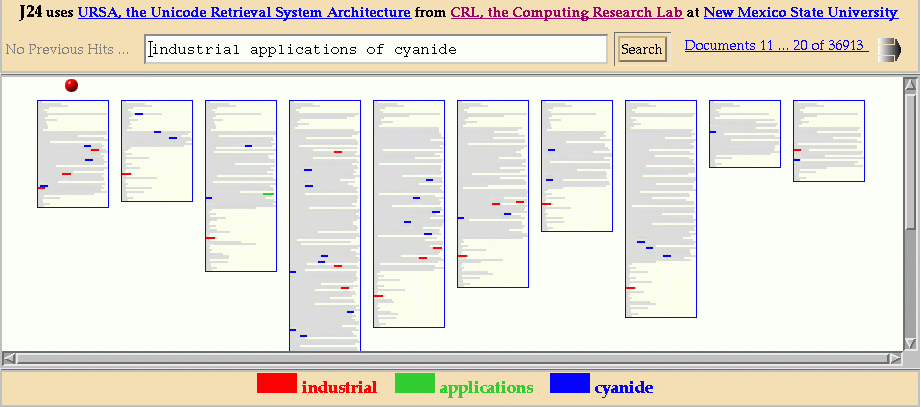
\includegraphics[width=\textwidth]{images/document_visualization/j24.png}
  \caption{``J24'' software's document overview with feature highlighting \\ \protect\autocite{ogdenDocumentThumbnailVisualizations1998a}}
  \label{fig:j24}
\end{figure}

\section*{Lexical Episode Plots}

A variation of this kind of document overview displays highlights beside the document outline also showing the ``topic'' of the highlight, it is called ``Lexical Episode Plots'' \autocite{el-assadyVisArgueVisualText2016,goldExploratoryTextAnalysis2015}.

\begin{figure}[H]
  \centering
  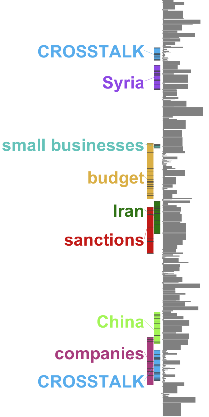
\includegraphics[height=0.5\textwidth]{images/document_visualization/topic-overview.png}
  \caption{``Lexical Episode Plots''\\ \protect\autocite{goldExploratoryTextAnalysis2015}}
  \label{fig:j24}
\end{figure}

\section*{Playing with font size}

\textcite{stoffelDocumentThumbnailsVariable2012} implement a combination of text highlighting along with font size variations for creating distorted thumbnails for previewing important document features.
I am a bit sceptical as to whether this would be a good thumbnail, the highlighted portions definitely show where key features are in the document, but the font size change does not contribute much at the document scale: most words are too small to be legible.
\textit{However} varying font size would be an interesting visualization for the Lime explanation's feature importance.

\begin{figure}[H]
  \centering
  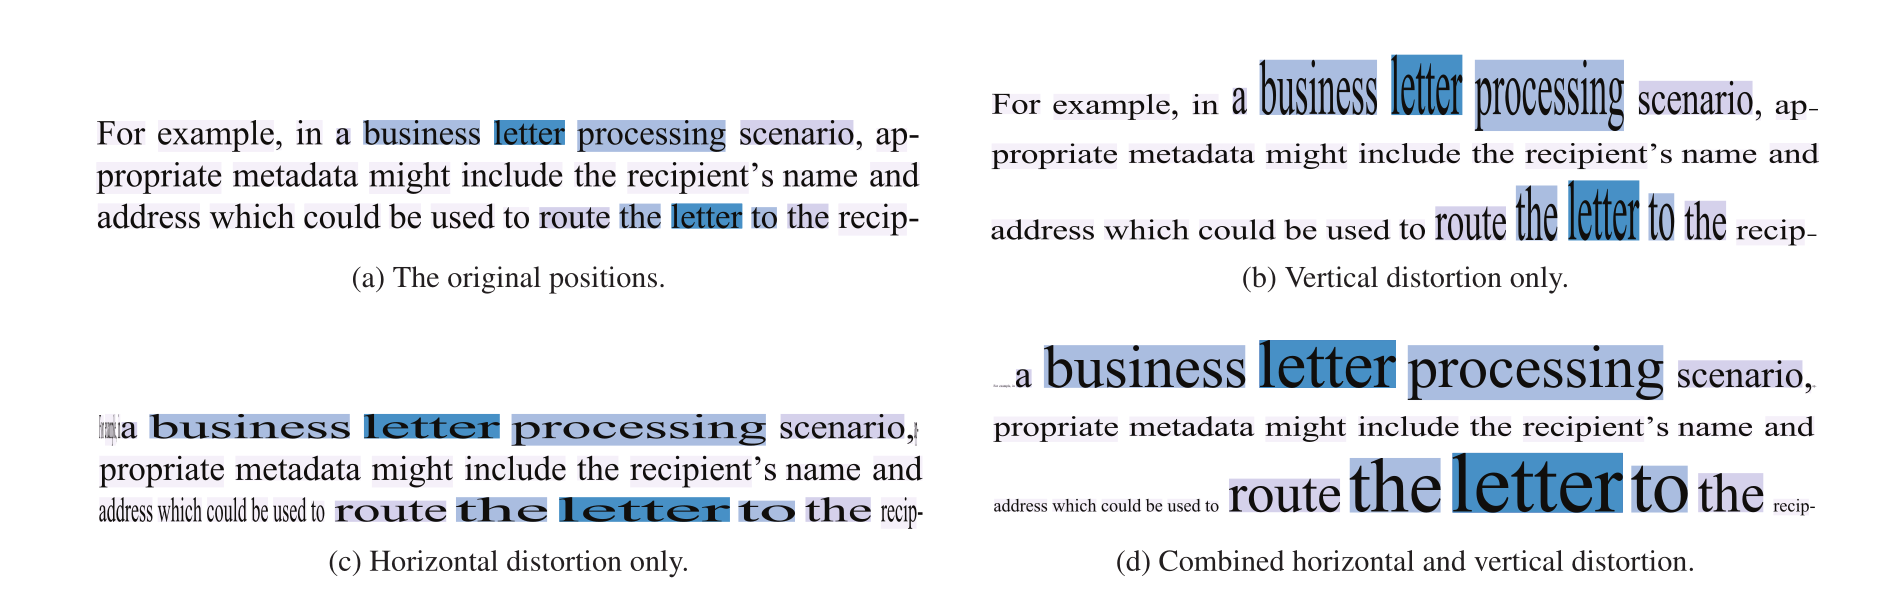
\includegraphics[width=\textwidth]{images/document_visualization/font-size.png}
  \caption{Adjusting font size for overview of important features \\ \protect\autocite{stoffelDocumentThumbnailsVariable2012}}
  \label{fig:font-size}
\end{figure}


\section*{Distortion}

This technique has many names and variants ``Document Lens'' \autocite{robertsonDocumentLens1993}, ``Fisheye'' view \autocite{greenbergFisheyeTextEditor1996} or ``hybrid continuous zoom`` \autocite{bartramContinuousZoomConstrained1995} with different implementations (see Figure \ref{fig:fisheyes}) they are part of a concept called ``Bifocal Display'' \autocite{apperleyBifocalDisplay}.

\begin{figure}[H]
  \centering
  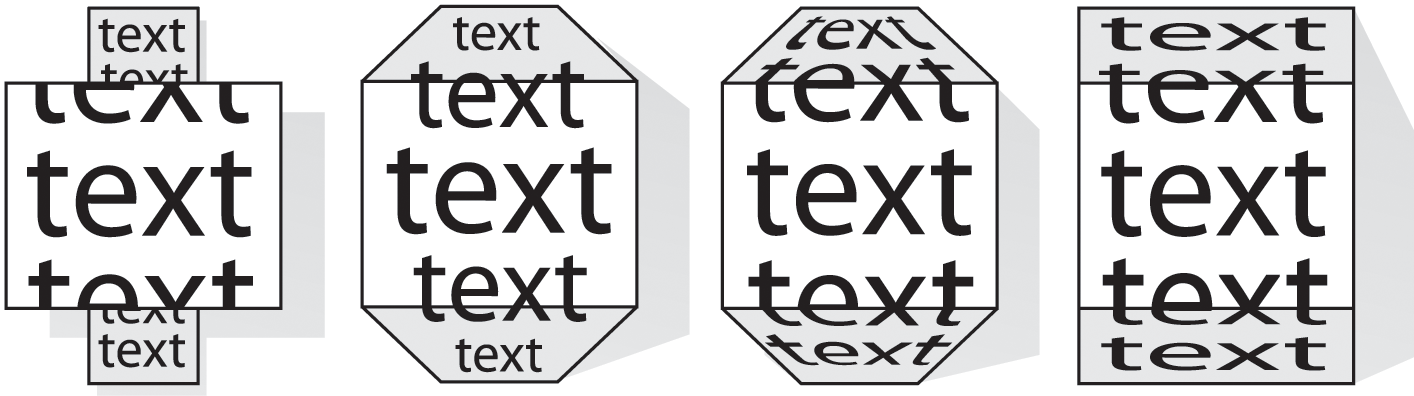
\includegraphics[width=\textwidth]{images/document_visualization/different-fisheyes.png}
  \caption{Different Fisheye views, from left to right: \\ Manhattan lens, zoomscapes, central perspective and parallel projection \\ \protect\autocite{baudischFishnetFisheyeWeb2004}}
  \label{fig:fisheyes}
\end{figure}

\textit{Circular Fisheye Distortion} is a circular ``magnifying glass'' effect visible in \textcite{bostockFisheyeGrid2019}. \textit{Cartesian Distortion} ``magnifies continuously so as to avoid local minification'' \autocite{bostockFisheyeDistortion2012}. The effect can also be limited to only one axis (vertical or horizontal) as seen in \textcite{pstuffaCartesianFisheyeDistortion2019}. In our case, Vertical Cartesian Distortion on a per line basis seems like an interesting visualization for document overview with emphasis on hovered lines. There is a D3js implementation of this effect (see the links above), it also seems like there is a React specific implementation of this text fisheye effect \autocite{zhongVincentdchanReactfisheye2019}.

\section{Related products}

Quite a few official government guidelines on the redaction of sensitive documents mention Adobe Acrobat as a go to tool for redacting text documents \autocite{thenationalarchivesRedactionToolkitPaper2016}.
Sometimes, the guidelines \textit{are} Adobe's guidelines for redaction \autocite{scottishgovernmentRedactingInformation2019}.

\subsection{PDF editors}

Adobe Acrobat is a well known PDF toolkit that notably enables sensitivity redaction of documents.
The principle is common: select text, click redact and browse a nested context menu to select an exemption (Figure \ref{fig:adobe-redaction}).

\begin{figure}[H]
    \centering
    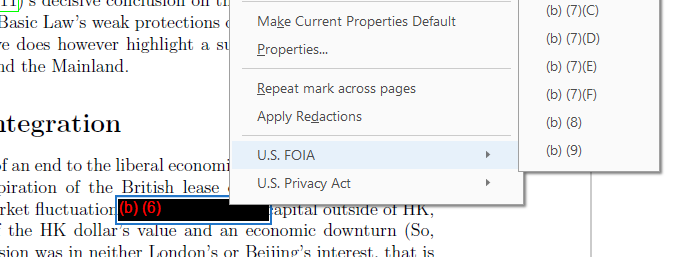
\includegraphics[width=\linewidth]{images/adobe_redaction.png}
    \caption{Adobe Acrobat redaction workflow}
    \label{fig:adobe-redaction}
\end{figure}

There are a variety of PDF editors, when they implement document redaction, they closely resemble this workflow.
For instance, Foxit PhantomPDF is another well known PDF editor that implements a strikingly similar context menu (Appendix \ref{fig:foxit-menu}) also allows for document wide redaction of a text selection (Appendix \ref{fig:foxit-redact-all}), something which Adobe implement quite poorly (Appendix \ref{fig:adobe-redact-all}).

%==================================================================================================================================
\chapter{Requirements}

\section{Scope}

\section{Functional Requirements (MoSCoW)}

% TODO reformulate this into something more formal
\begin{minipage}[t]{.5\linewidth}
    \centerline{\textbf{Must Have}}
    \begin{itemize}
        \item document Set creation and deletion
        \item within a set, plaintext document creation and deletion
        \item for a document, binary sensitivity classification (sensitive or not?)
        \item explanation for aforementioned classifications
        \item user binary classification of a document (sensitive or not?)
        \item for a set of document, overall sensitivity statistics (number of sensitive documents etc…)
        \item for a set of documents, ordered of documents by sensitivity
        \item User redactions of a document with text highlighting, with possible edits and save functionality
        \item final redacted document exporting
        \item documentation for API
    \end{itemize}
\end{minipage}
\hfill
\noindent
\begin{minipage}[t]{.5\linewidth}
    \centerline{\textbf{Should Have}}
    \begin{itemize}
        \item user redactions helper (highlight all instances of redacted text, could do this on a document set level)
        \item for a document, suggest redaction of sensitive elements
        \item fulltext document search
    \end{itemize}
\end{minipage}

\vspace{0.5cm}

\begin{minipage}[t]{.5\linewidth}
    \centerline{\textbf{Could Have}}
    \begin{itemize}
        \item extract entities from document and display them (spaCy)
        \item possibility of using different text Classifiers (what for?)
        \item documentation for API SDK
        \item documentation for frontend
        \item specified and enforced document upload limitations (number and size of documents)
        \item reviewer authentication
    \end{itemize}
\end{minipage}
\hfill
\noindent
\begin{minipage}[t]{.5\linewidth}
    \centerline{\textbf{Would Have}}
    \begin{itemize}
        \item handle more than plain text files (PDF, Word etc…)
        \item specified and enforced document size and count upload limits
        \item ``Loopback Learning'' user redactions help improve future predictions
        \item deployed web application
    \end{itemize}
\end{minipage}

\section{(non)Functional definition}

user study

\section{Wireframing}

\begin{figure}[H]
    \centering
    \begin{subfigure}[b]{\linewidth}
        \centering
        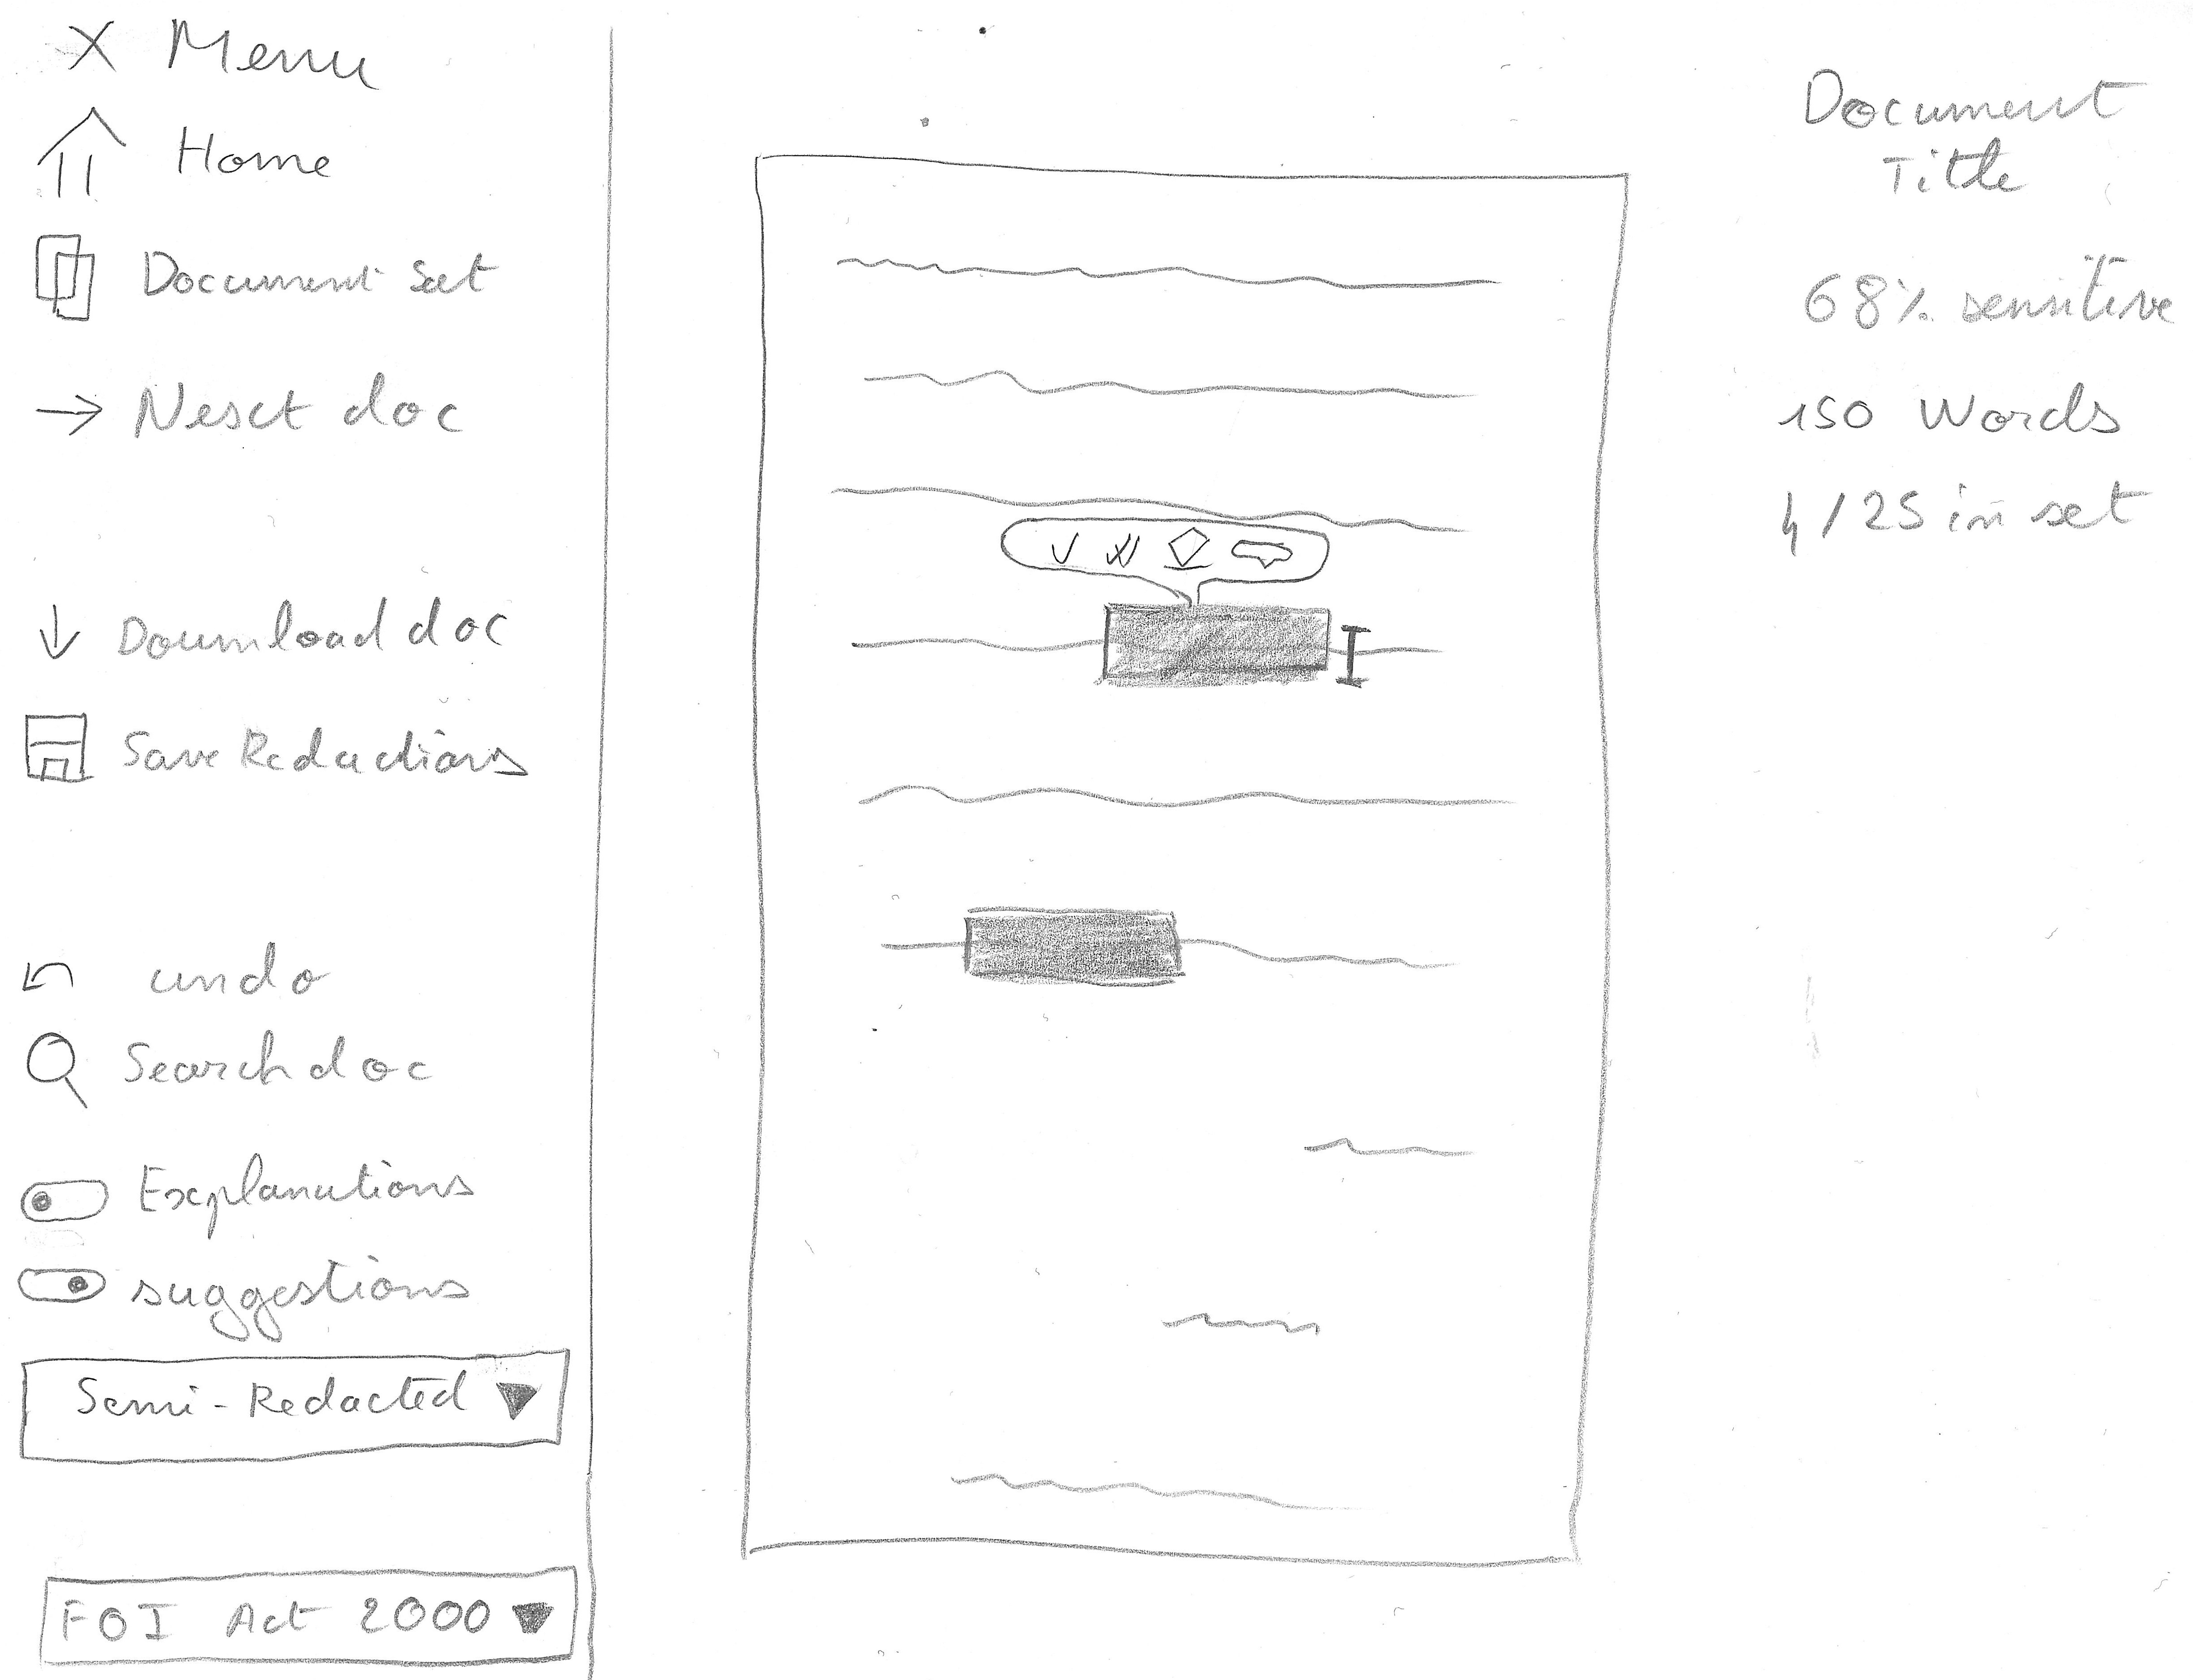
\includegraphics[width=0.6\linewidth]{images/wireframes/doc_view.jpg}
        \caption{Document View Wireframe}
        \label{fig:document-wireframe}
    \end{subfigure}
    \begin{subfigure}[b]{\linewidth}
        \begin{subfigure}[b]{0.5\linewidth}
            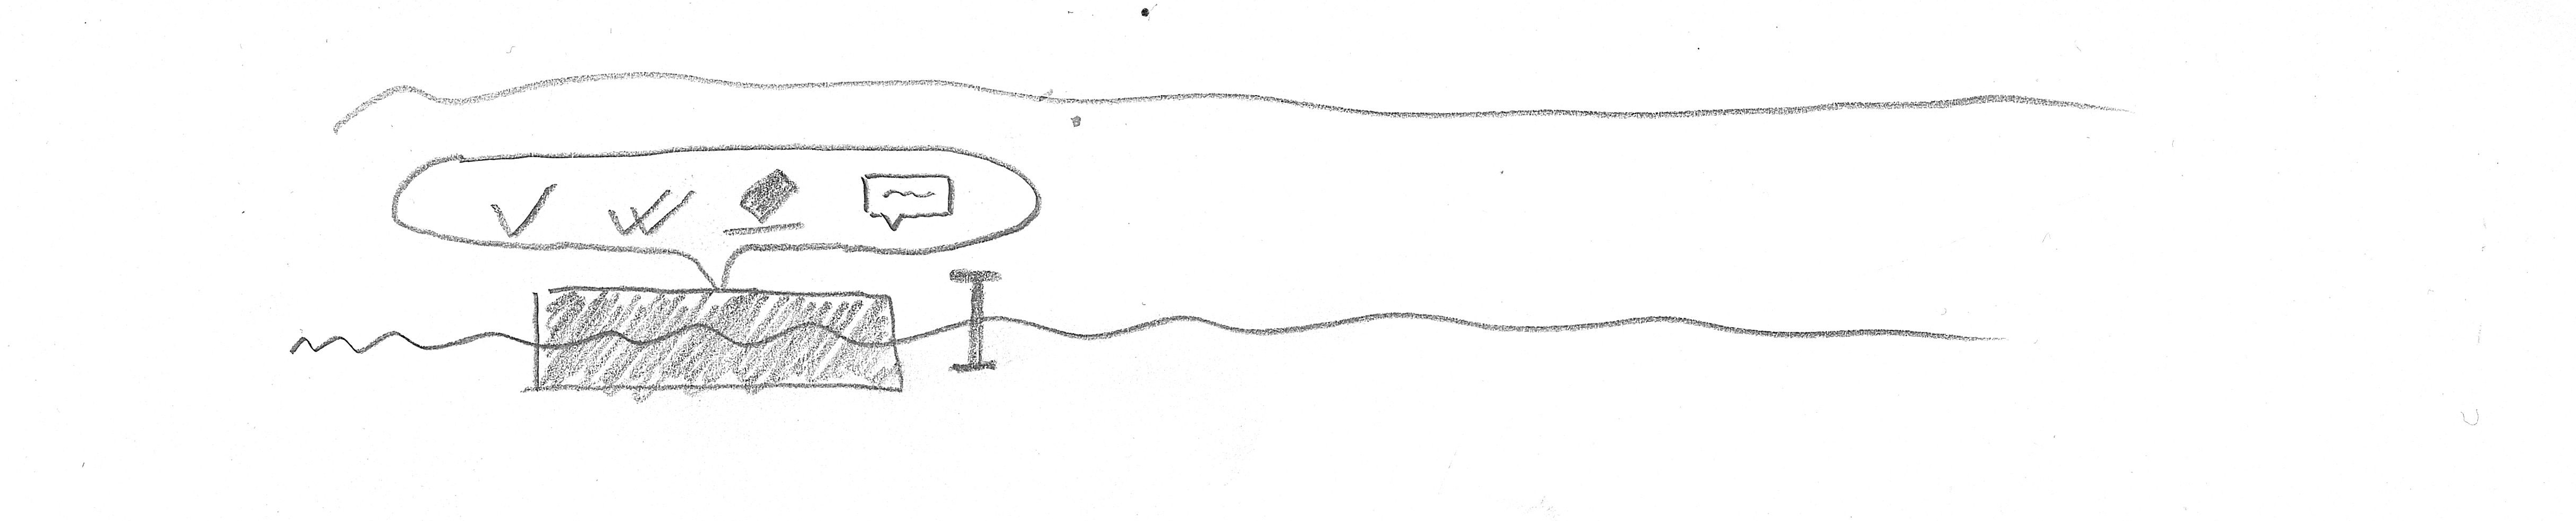
\includegraphics[width=\linewidth]{images/wireframes/tooltip.jpg}
            \caption{minimized tooltip wireframe}
            \label{fig:tooltip-wireframe}
        \end{subfigure}
        \begin{subfigure}[b]{0.4\linewidth}
            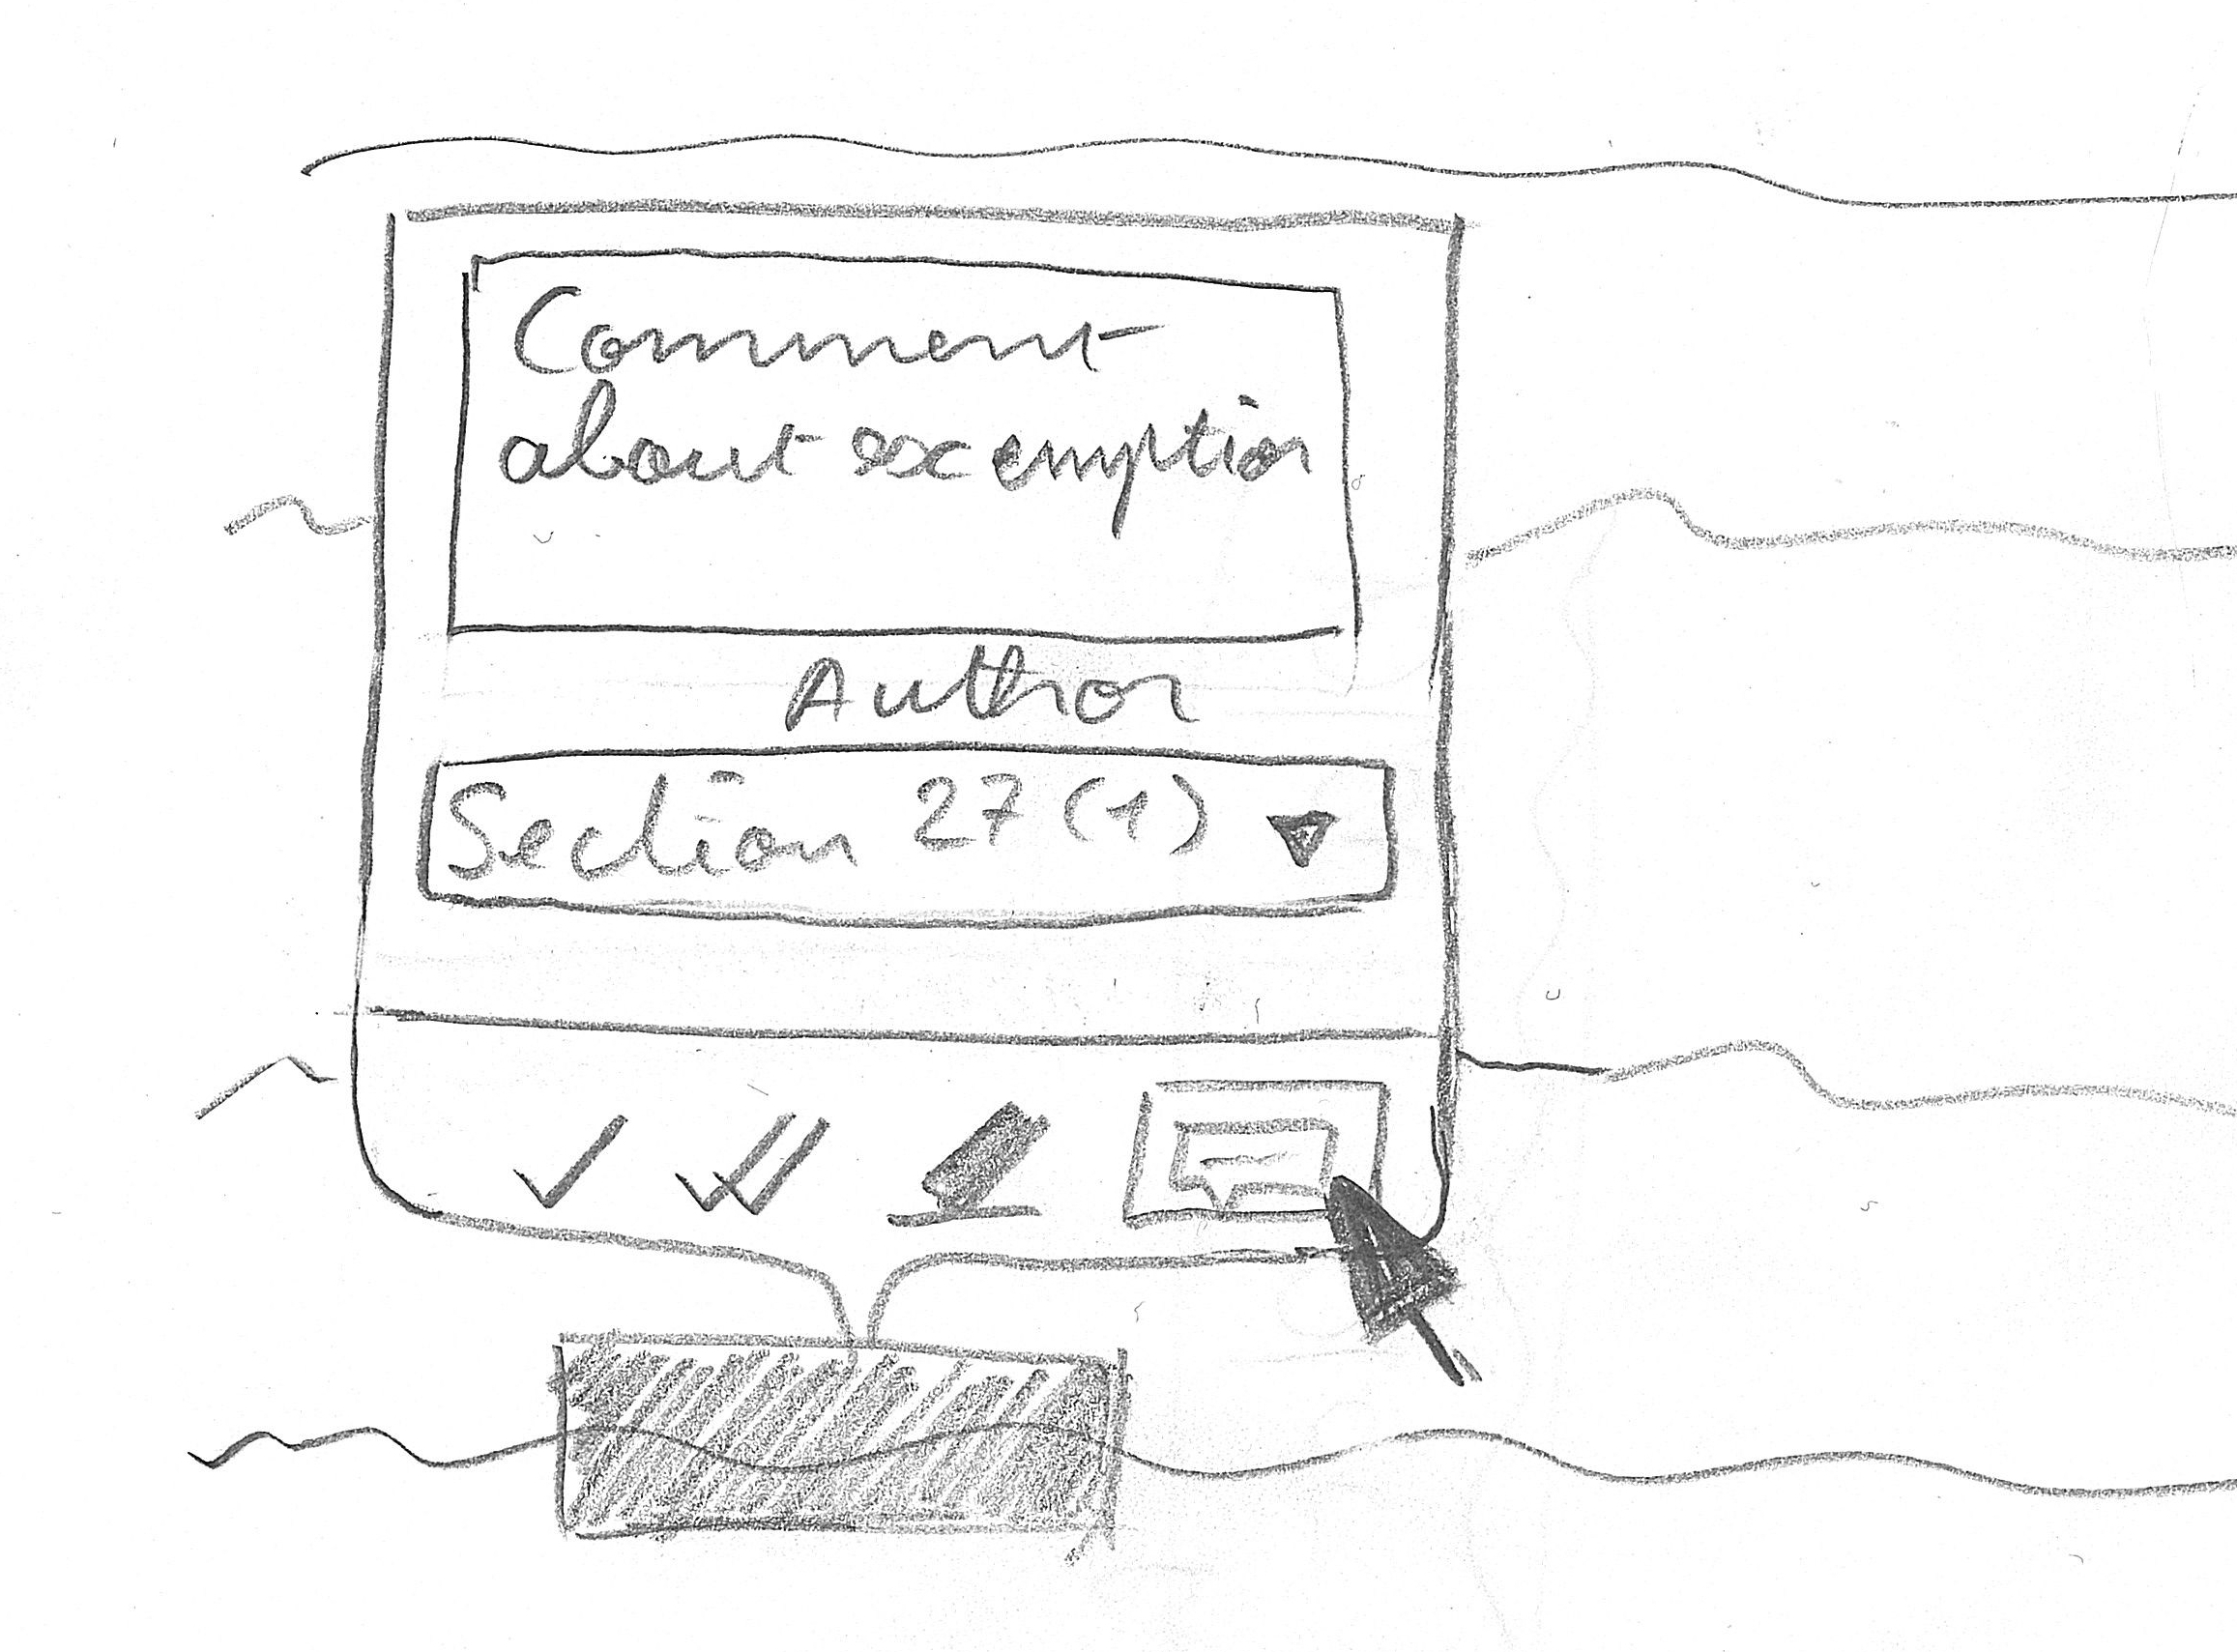
\includegraphics[width=\linewidth]{images/wireframes/tooltip_comment.jpg}
            \caption{Expanded tooltip wireframe}
            \label{fig:expanded-tooltip-wireframe}
        \end{subfigure}
    \end{subfigure}
    \caption{Selection of some of the Wireframes drawn up during the design process}
    \label{fig:wireframes}

\end{figure}


%==================================================================================================================================
\chapter{Design}

link back to requirements

choice of technologies

\section{Application Structure and Technology stack}

\section{Machine Learning Model}

% TODO this sounds too much like a list

We used the Scikit-Learn library to implement our Machine Learning Models \autocite{pedregosaScikitlearnMachineLearning2011}, for performance reasons, we replaced its SVC implementation with a drop-in parallel replacement ``ThunderSVM'' which can operate on multicore CPUs or CUDA enabled GPUs \autocite{wenThunderSVMFastSVM2018}.
We resampled our highly unbalanced dataset with an extension to Scikit-Learn: ``imblearn'' which implements common resampling techniques\autocite{lemaitreImbalancedlearnPythonToolbox2017}.
% TODO elaborate on this, how it works
In order to provide explanations for our model's predictions utilized techniques implemented by Lime which provides per-feature weights explaining the feature's contribution to the final classification \autocite{ribeiroWhyShouldTrust2016a}.

% TODO 
\autocite{lundbergUnifiedApproachInterpreting2017a} Shapley values


\subsection{OpenAPI specification and generator}

``The OpenAPI Specification is a community-driven open specification within the OpenAPI Initiative, a Linux Foundation Collaborative Project.'' \autocite{OAIOpenAPISpecification2020}. 
% TODO elaborate a bit more on this
It is an increasingly popular formal definition of a REST API contract. 
Its precision and specificity is such that it has allowed powerful tools to expand it.
Notably, the OpenAPI generator \autocite{OpenAPIToolsOpenapigenerator2020} which, given an OpenAPI specification, allows for the \textit{automatic} generation of API server code in more than 40 languages and API client code in more than 50.
Hence, we chose to write our API specification in OpenAPI format \textit{before} developing the API.
This allowed us to generate boilerplate API server code and a full fledged API client with only the precise documentation.


\section{API Server}

Most of our data science tools are written in Python which is why we selected it to write our API server.
The question of the choice of framework, remained, specifically since the OpenAPI generator allows for the generation of Python Server code with 3 different frameworks


\section{Frontend}

%==================================================================================================================================
\chapter{Implementation}

show coponennt code and how it gets data from backend

show lime explanations generation

key ``features'' code overview


\begin{itemize}
    \item Hands on SkLearn framework, experimented with different text pre-processing techniques and classifiers to build a Pipeline to classify textual documents into either sensitive or not sensitive categories
    \item overview of Machine Learning model explanation techniques, successfully implemented the Lime explainer, tried to use the SHAP explainer, but was unsuccessful
    \item Explore text document storage, looked at Terrier, ElasticSearch to finally settle on MongoDB
    \item Packaged SkLearn classifier into Python Flask API with OpenAPI specification
    \item created Javascript API Client from code generated from OpenAPI specification
    \item hands on ReactJS Javascript frontend framework, implemented a document browsing, viewing and upload frontend
    \item added text redaction feature to mark sections as sensitive with a label explaining why it is deemed sensitive
    \item implemented Lime Model explanations in Python backend, exposed them to the Flask API and created a frontend "in text" visualization of these sensitivities
    \item Research Document visualization techniques (literature review)
    \item created a populator script to load and classify all documents
    \item graph visualization of feature contribution to the classification and other UI tweaks
\end{itemize}

%==================================================================================================================================
\chapter{Evaluation}

We conducted a user evaluation in order to evaluate the effectiveness of our application in helping reviewers conduct a sensitivity review. We sought to answer a handeful of research questions.

\begin{itemize}
    \item Firstly, does our visualization of predicted document sensitivity and explanation features help reviewers conduct a sensitivity review faster?
    \item Secondly, does it improve the accuracy of the sensitivity review process.
    \item Lastly, does it improve reviewers' confidence in the completeness of their sensitivity review
\end{itemize}

\section{Preparations and Experimental Setup}

Our collection is a set of 3801 Government documents relating to International Activities sensitivity reviewed by government sensitivity reviewers.
The ground truth for document sensitivity was established with respect to sections 40 (S40) (Personal Information) and 27 (S27) (International Relations) of the Freedom of Information Act (FOIA).

Due to our lack of access to expert document reviewers, we conducted our study thanks to students either from an academic politics background or with International Relations awareness.
We focused on identifying ``Personal Information'' exceptions to the FOIA which we deemed more ``attainable'' given our non-expert test subjects.

Our dataset contains 289 documents with S40 exemptions, we split the collection in order to obtain a stratified sample ``test set'' 20\% the size of the entire collection.
We vectorized the remaining 80\% ``train set'' using Scikit-Learn's \verb|TfidfVectorizer| \autocite{pedregosaScikitlearnMachineLearning2011}.
We resampled the resulting vectors to achieve better class balance with imblearn's \verb|SMOTEENN|, a combination of majority class downsampling and minority class upsampling \autocite{lemaitreImbalancedlearnPythonToolbox2017}.
We used the resulting vectorized and resampled documents to train a GPU accelerated SVC \autocite{wenThunderSVMFastSVM2018} for binary classification of documents depending on whether or not they contain sensitive information.

Due to time constraints, we sampled only sampled documents to review from the test set that were under 2000 characters.
We then selected both sensitive and non-sensitive documents in order to represent every category of the confusion matrix for the classifier with the following counts:

\begin{table}[H]
    \begin{tabular}{l ll}
                                & Actually non-sensitive & Actually Sensitive \\
        Predicted non-sensitive & 3                      & 1                  \\
        Predicted Sensitive     & 1                      & 1
    \end{tabular}
    \caption{Count of selected documents in the classifier's confusion matrix}
    \label{tab:confusion-matrix-selection}
\end{table}


We sampled test documents accordingly twice: once for each User Interface (UI) used in the evaluation.
One interface \textit{test mode 1} (Figure \ref{fig:test-mode-1}) is a simplified version of the final interface containing the classification prediction and the accompanying explanations.
The other, \textit{test mode 2} (Figure \ref{fig:test-mode-2}) is a stripped down version that only displays the document, and the manual redaction tools (document title and sensitivity type selection).
Our reviewers reviewed documents with both interfaces, the first interface displayed was selected randomly.


\begin{figure}[H]
    \centering
    \begin{subfigure}[b]{0.7\textwidth}
        \centering
        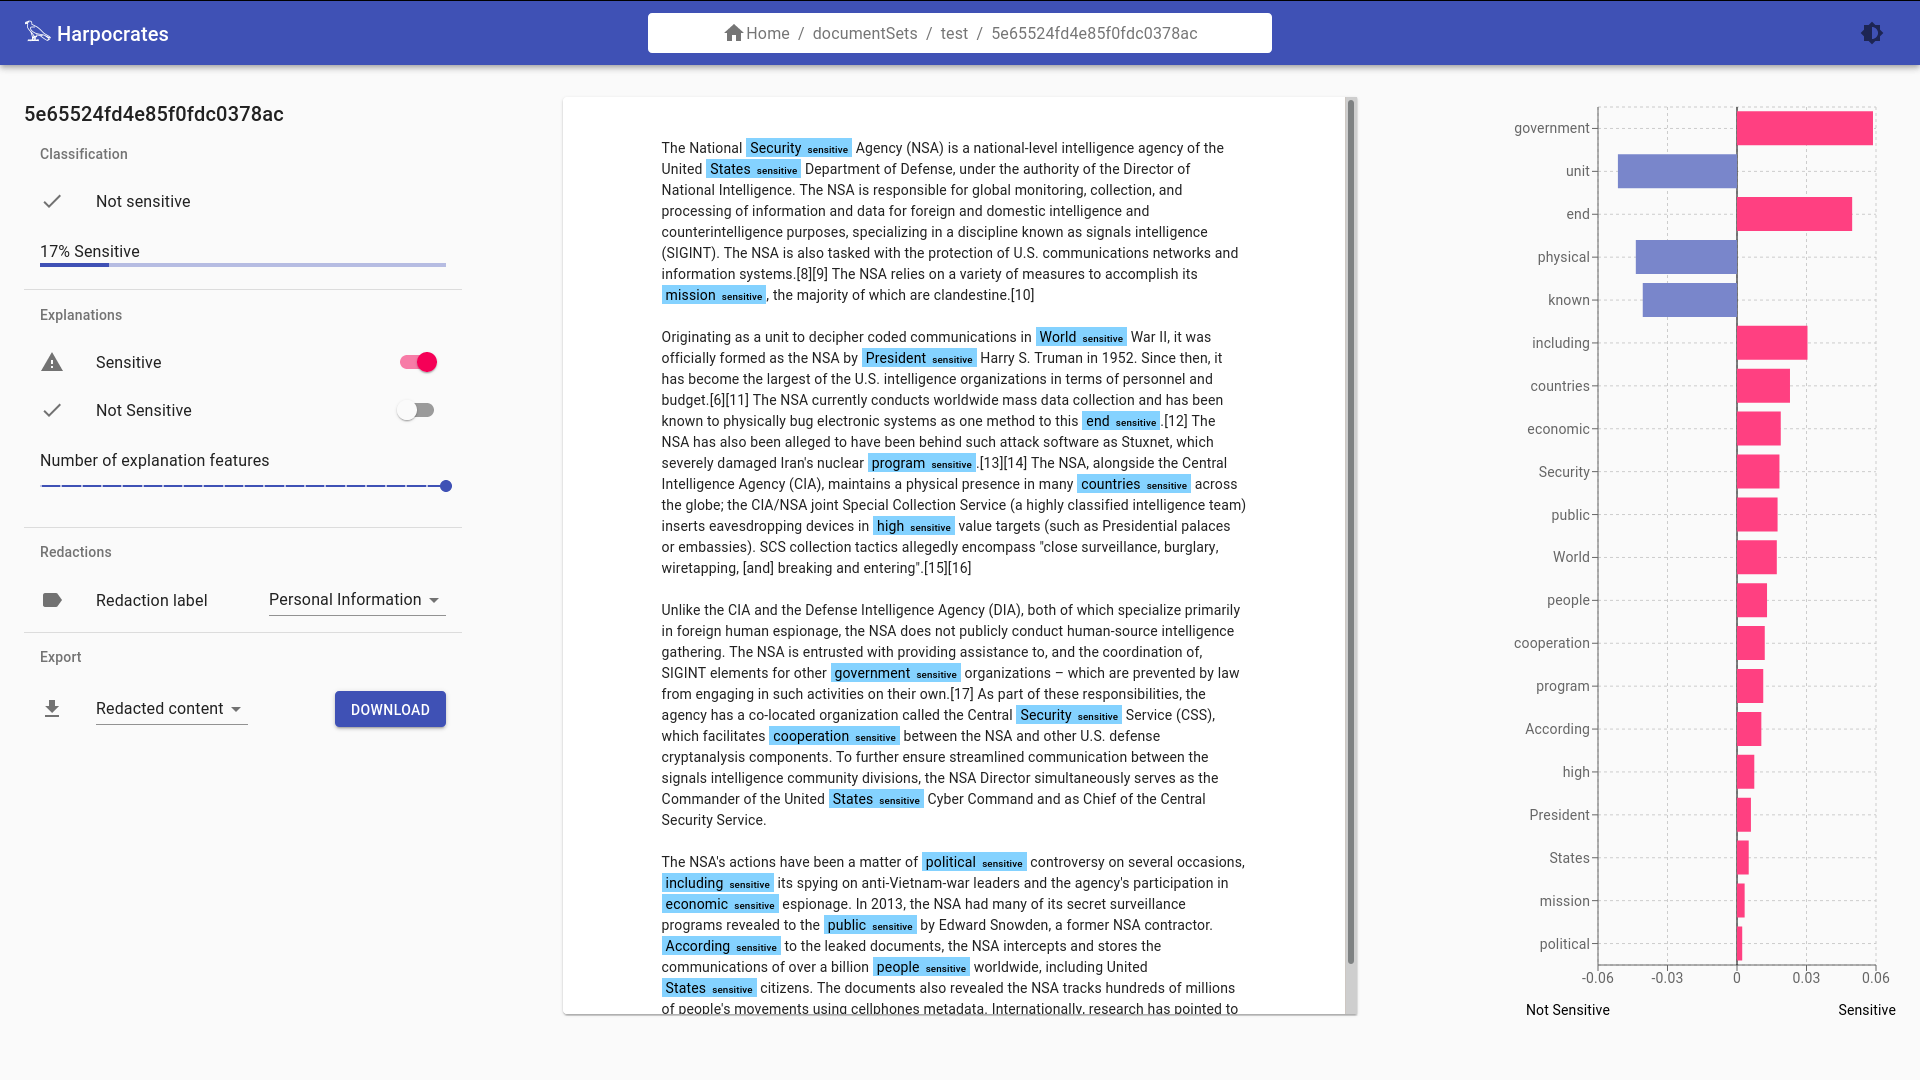
\includegraphics[width=\linewidth]{images/ui_test_mode_1.png}
        \caption{Test mode 1}
        \label{fig:test-mode-1}
    \end{subfigure}


    \begin{subfigure}[b]{0.7\textwidth}
        \centering
        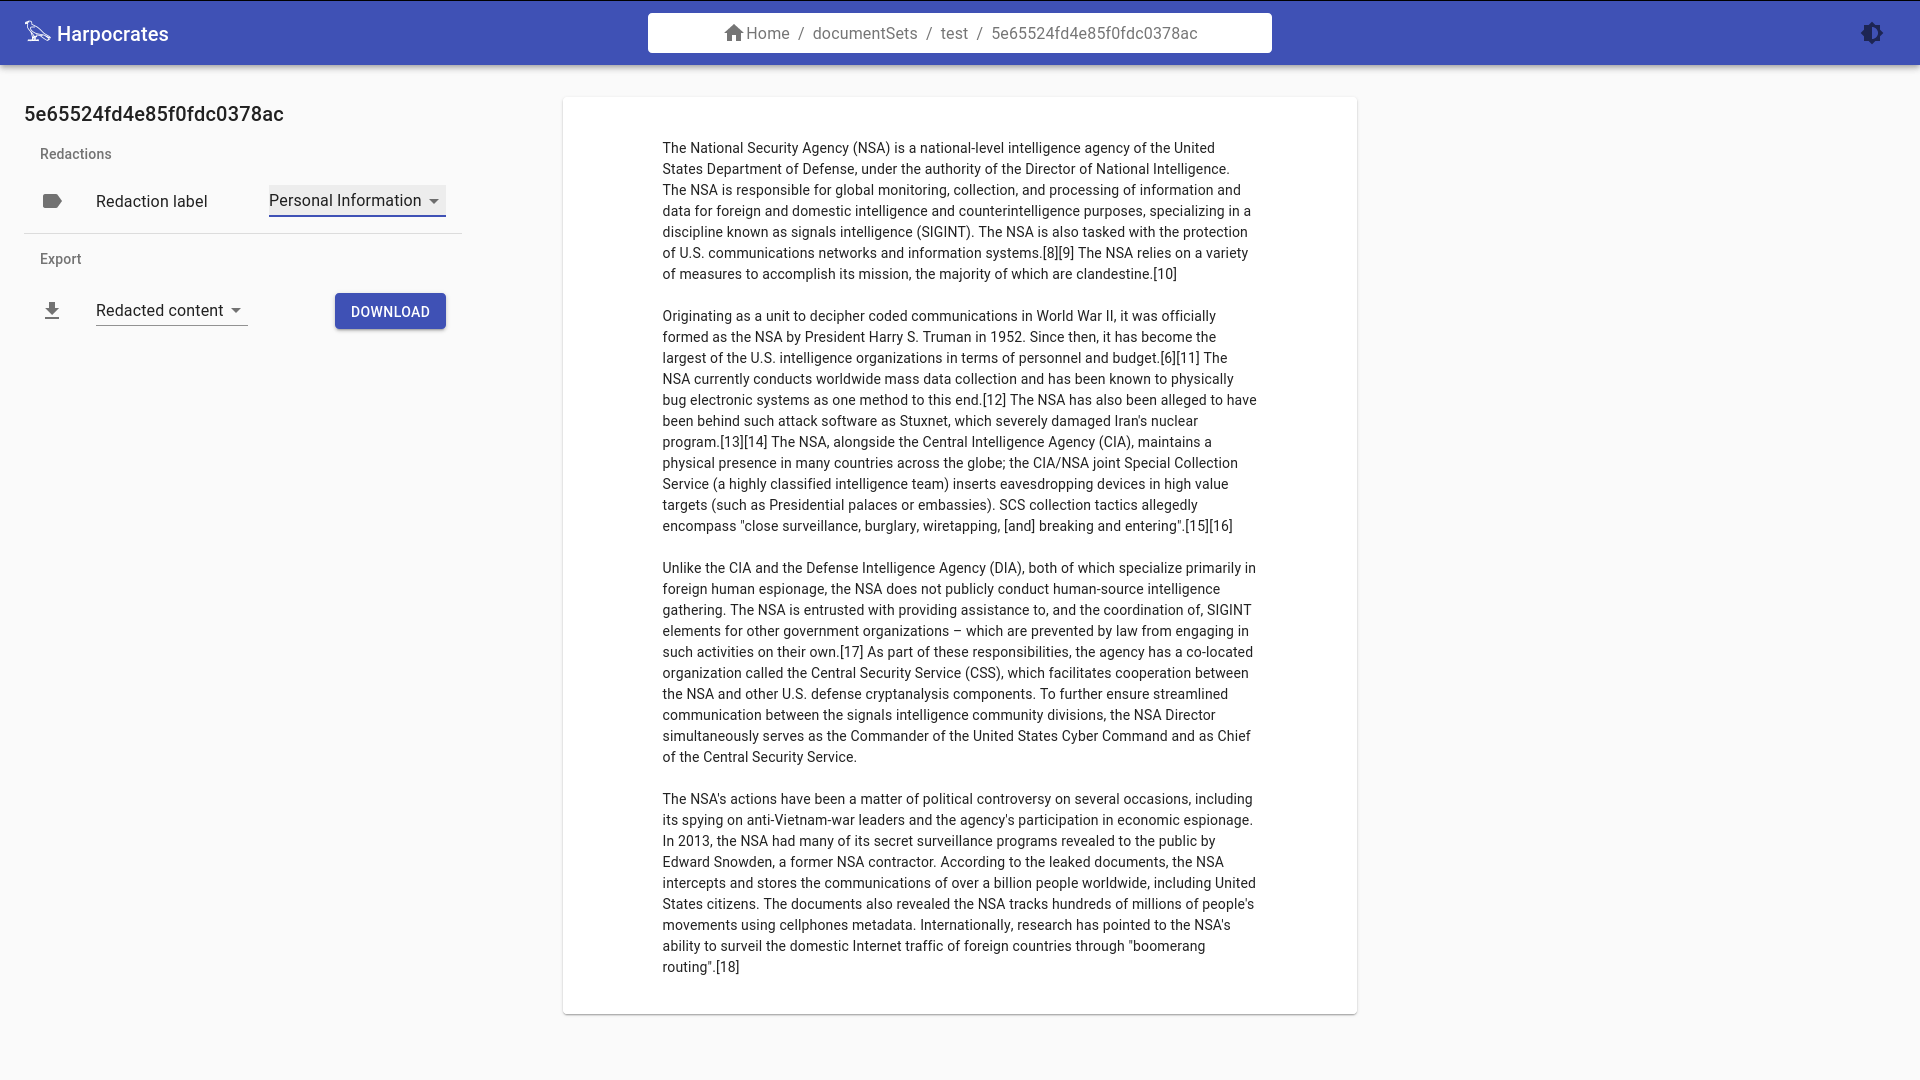
\includegraphics[width=\linewidth]{images/ui_test_mode_2.png}
        \caption{Test mode 2}
        \label{fig:test-mode-2}
    \end{subfigure}
    \caption{The two test modes used for evaluation}
    \label{fig:test-modes}
\end{figure}

% TODO put questionnaire in appendix 
% TODO link questionnaire here
Lastly, after the review of a batch of documents with each interface, a questionnaire was handed out to the testers

\section{Evaluation}

As mentioned, each user will be asked to review one collection of 6 documents for personal information sensitivities (FOIA Section 27) per user interface

The independent variables will a set of two user interfaces: with and without the predicted classification and explanations (more details below) which all users will both use. We will measure multiple dependent variables:

\begin{itemize}
    \item Firstly, we will measure the time to review an entire collection with each interface.
    \item Secondly we will record the accuracy of each reviewer on each interface for all documents.
    \item Lastly, we will evaluate the confidence of the reviewers after using each interface with a Likert scale in the questionnaires.
\end{itemize}




Research questions
dependent/indepdent variables
UI variations
experimental setup
document, subject seleciton


results


link back to requirements
how have they been met
unit testing




%==================================================================================================================================
\chapter{Conclusion}


requirements I've met


reflections

future work

%==================================================================================================================================
%
% 
%==================================================================================================================================
%  APPENDICES  

\begin{appendices}
    \chapter{PDF Editors}
    \section{PhantomPDF context menu}
    \label{fig:foxit-menu}
    \begin{figure}[H]
        \centering
        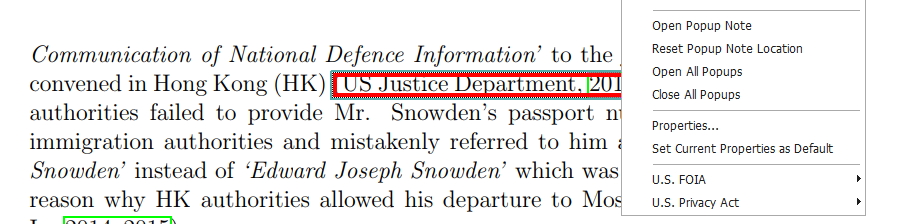
\includegraphics[width=\linewidth]{images/foxit_redaction.png}
    \end{figure}
    \section{PhantomPDF redact all}
    \label{fig:foxit-redact-all}
    \begin{figure}[H]
        \centering
        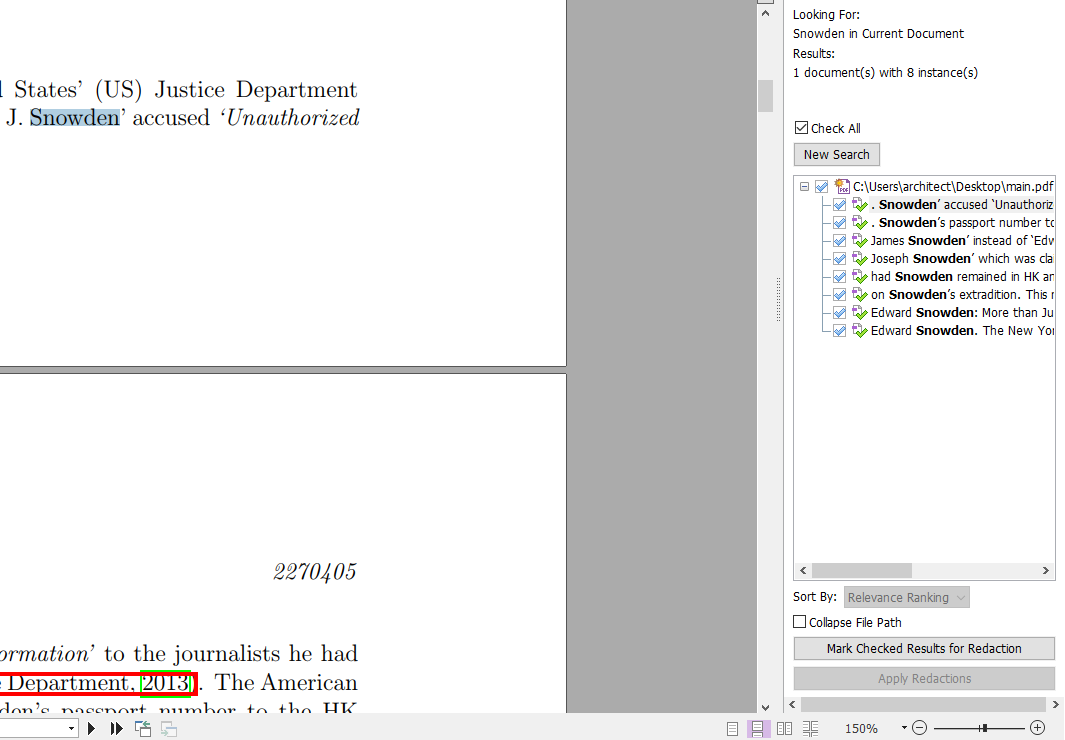
\includegraphics[width=\linewidth]{images/foxit_redact_all.png}
    \end{figure}
    \section{Adobe Acrobat redact all}
    \label{fig:adobe-redact-all}
    \begin{figure}[H]
        \centering
        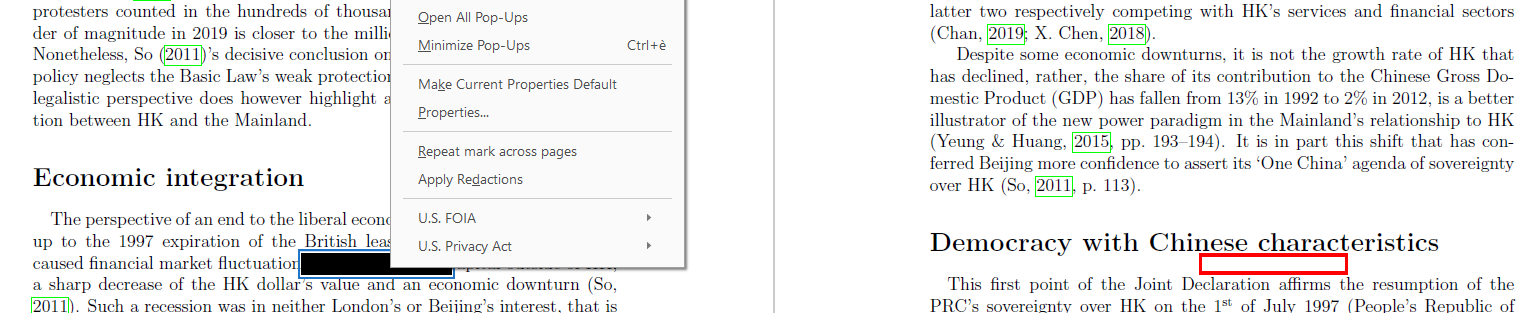
\includegraphics[width=\linewidth]{images/adobe_redact_all.png}
    \end{figure}
    \chapter{Wireframes}
    \section{Homepage}
    \begin{figure}[H]
        \centering
        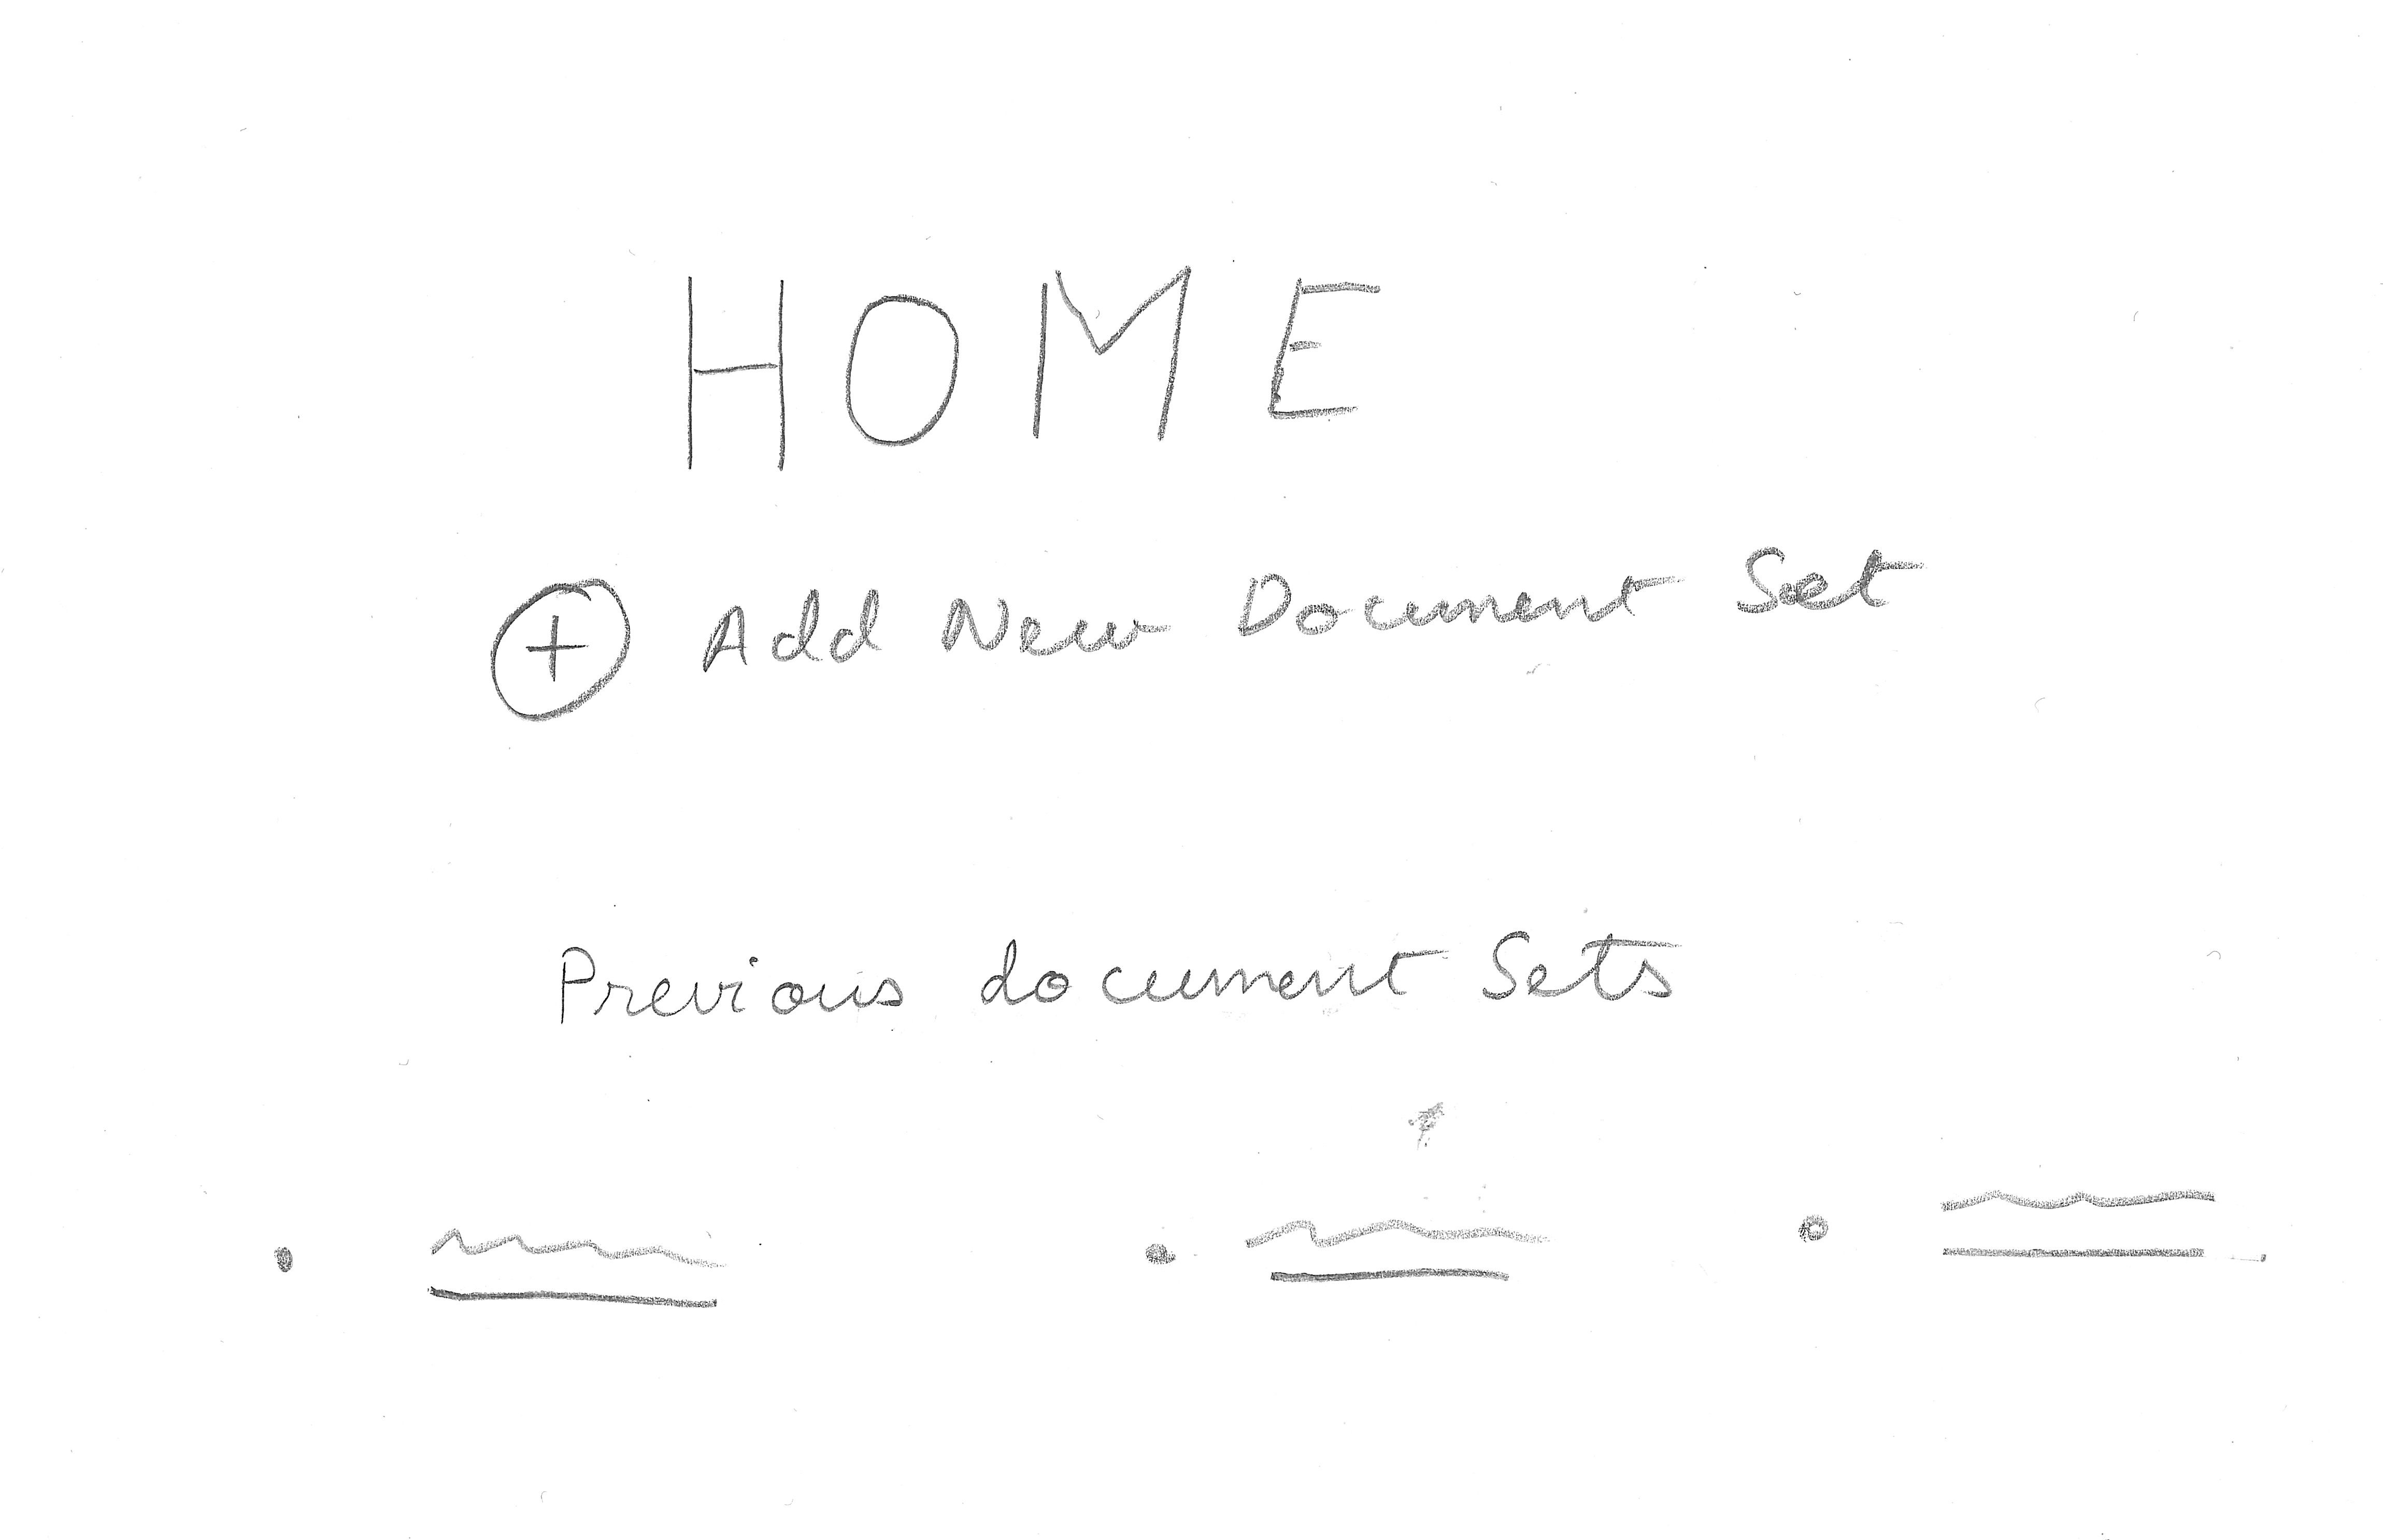
\includegraphics[width=\linewidth]{images/wireframes/home.jpg}
    \end{figure}
    \section{Set View}
    \begin{figure}[H]
        \centering
        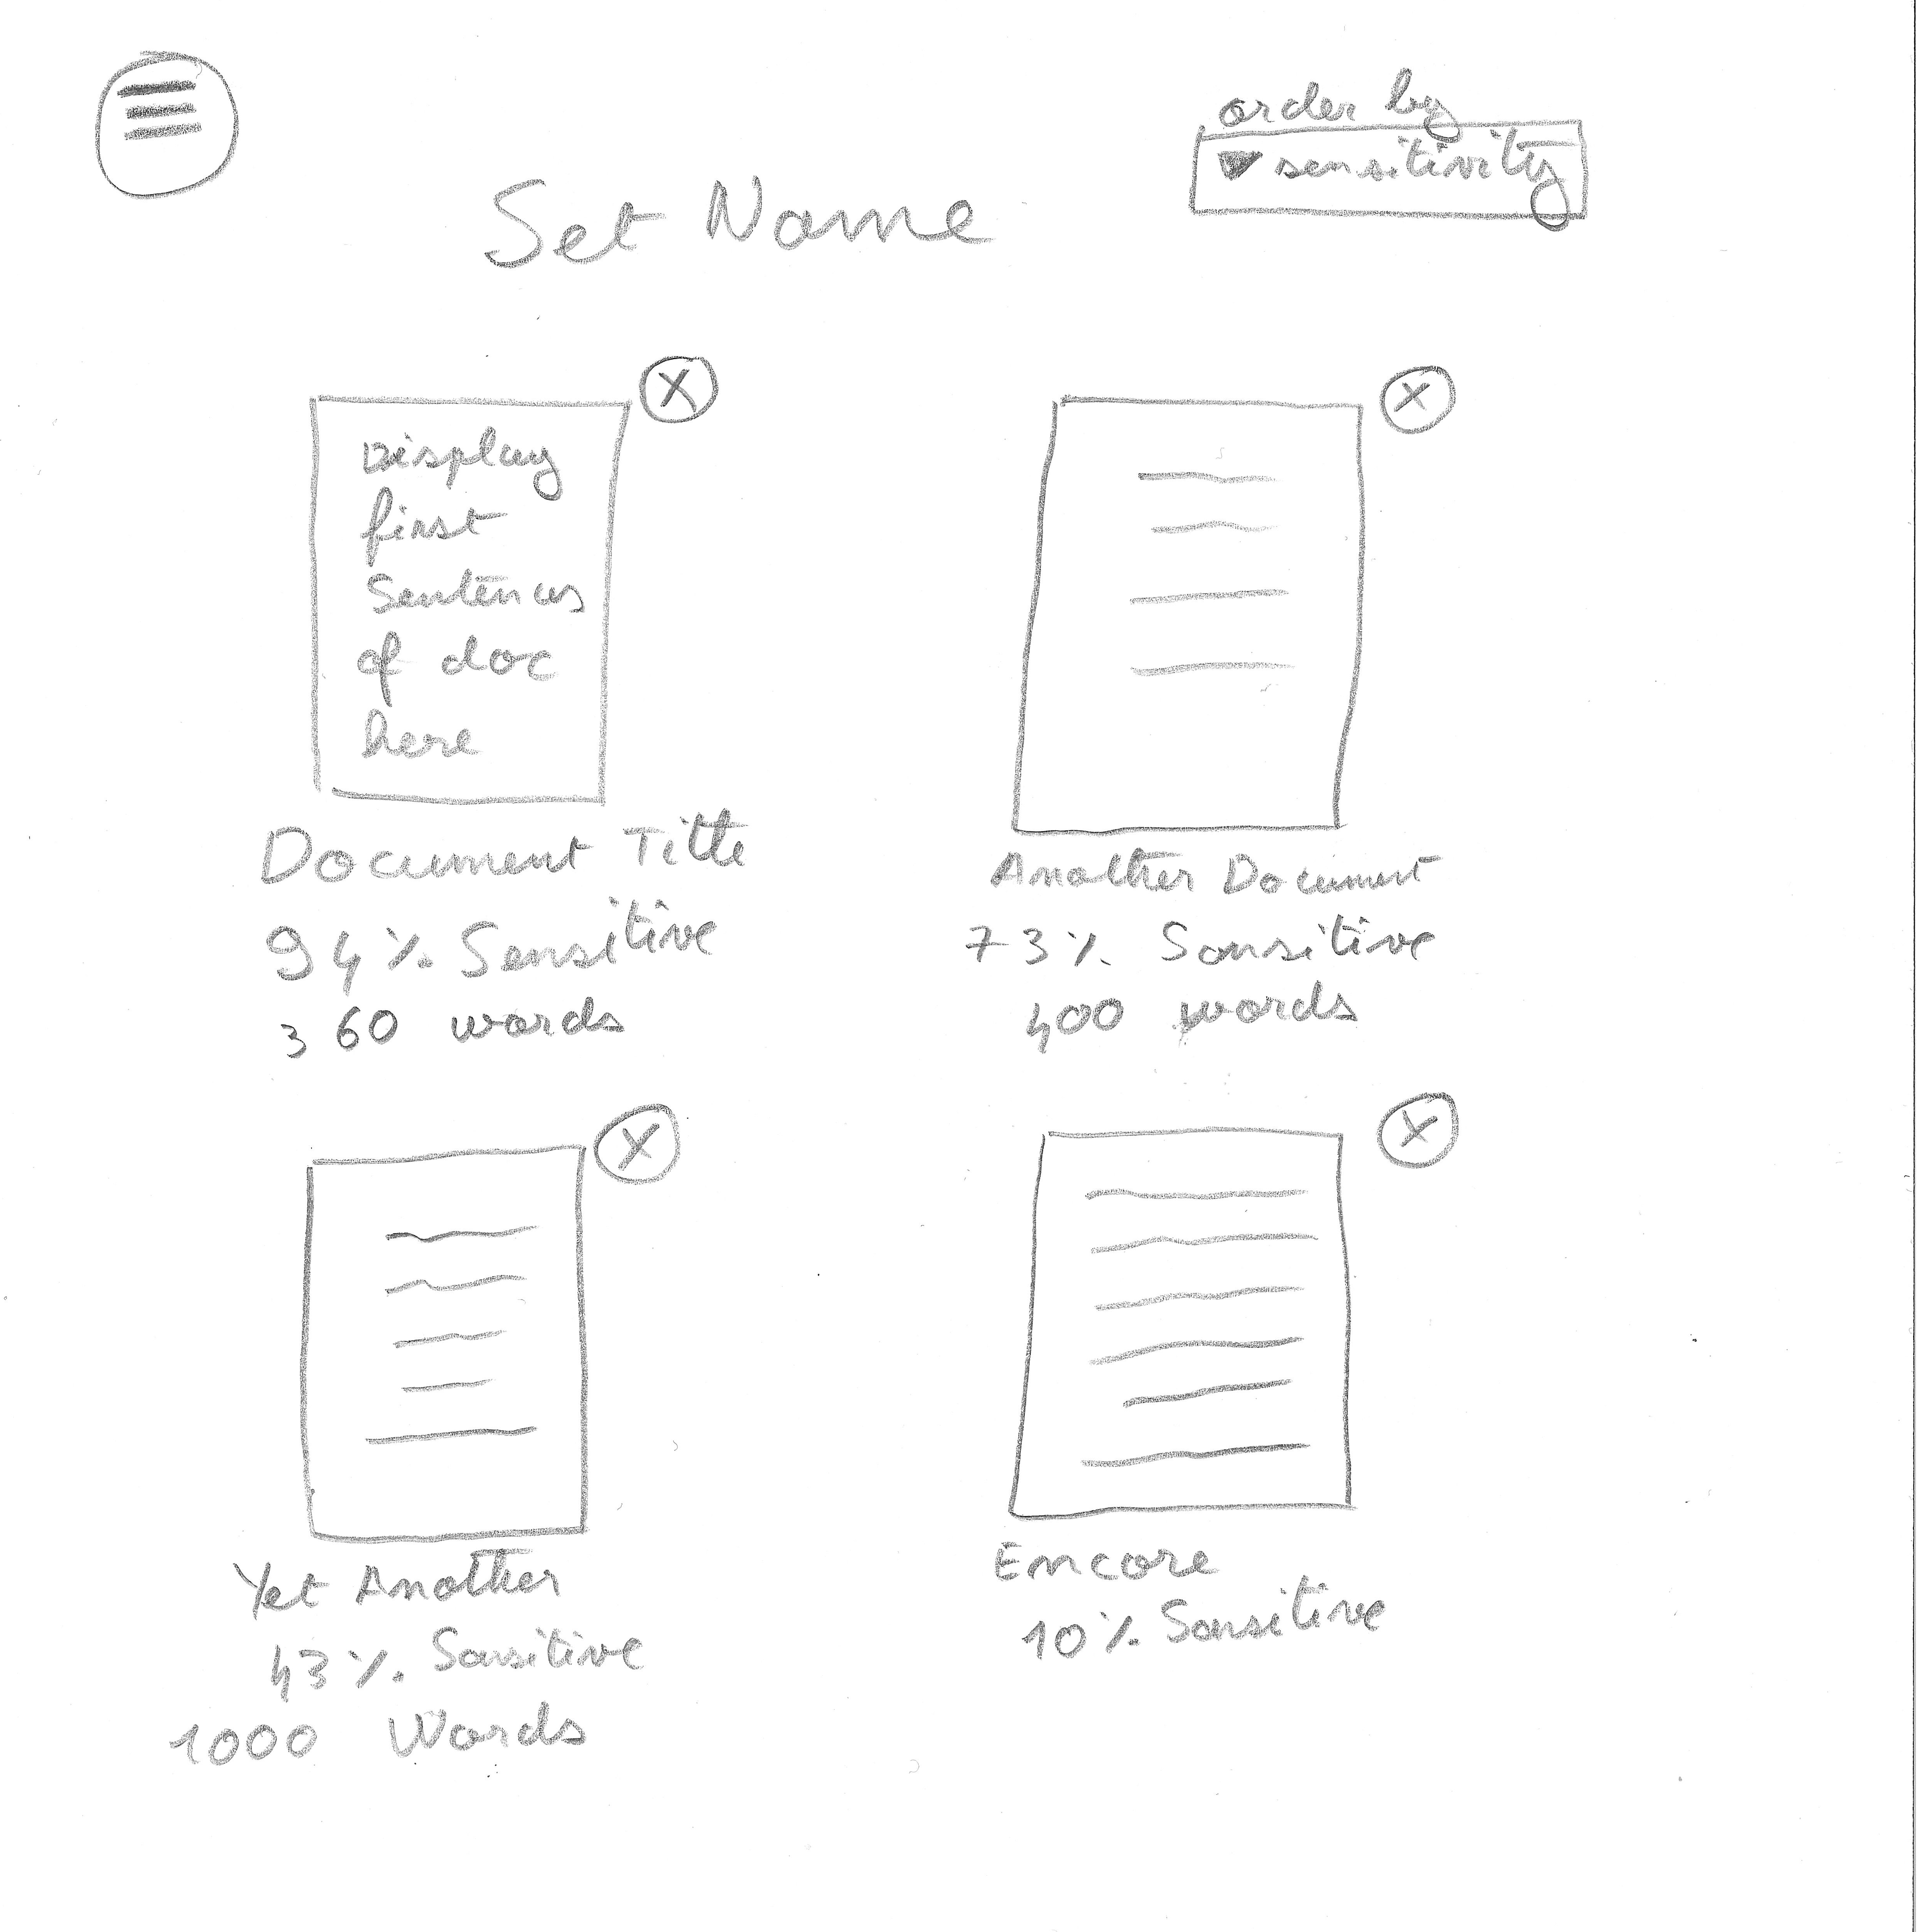
\includegraphics[width=0.8\linewidth]{images/wireframes/set.jpg}
    \end{figure}
    \section{Set View - menu open}
    \begin{figure}[H]
        \centering
        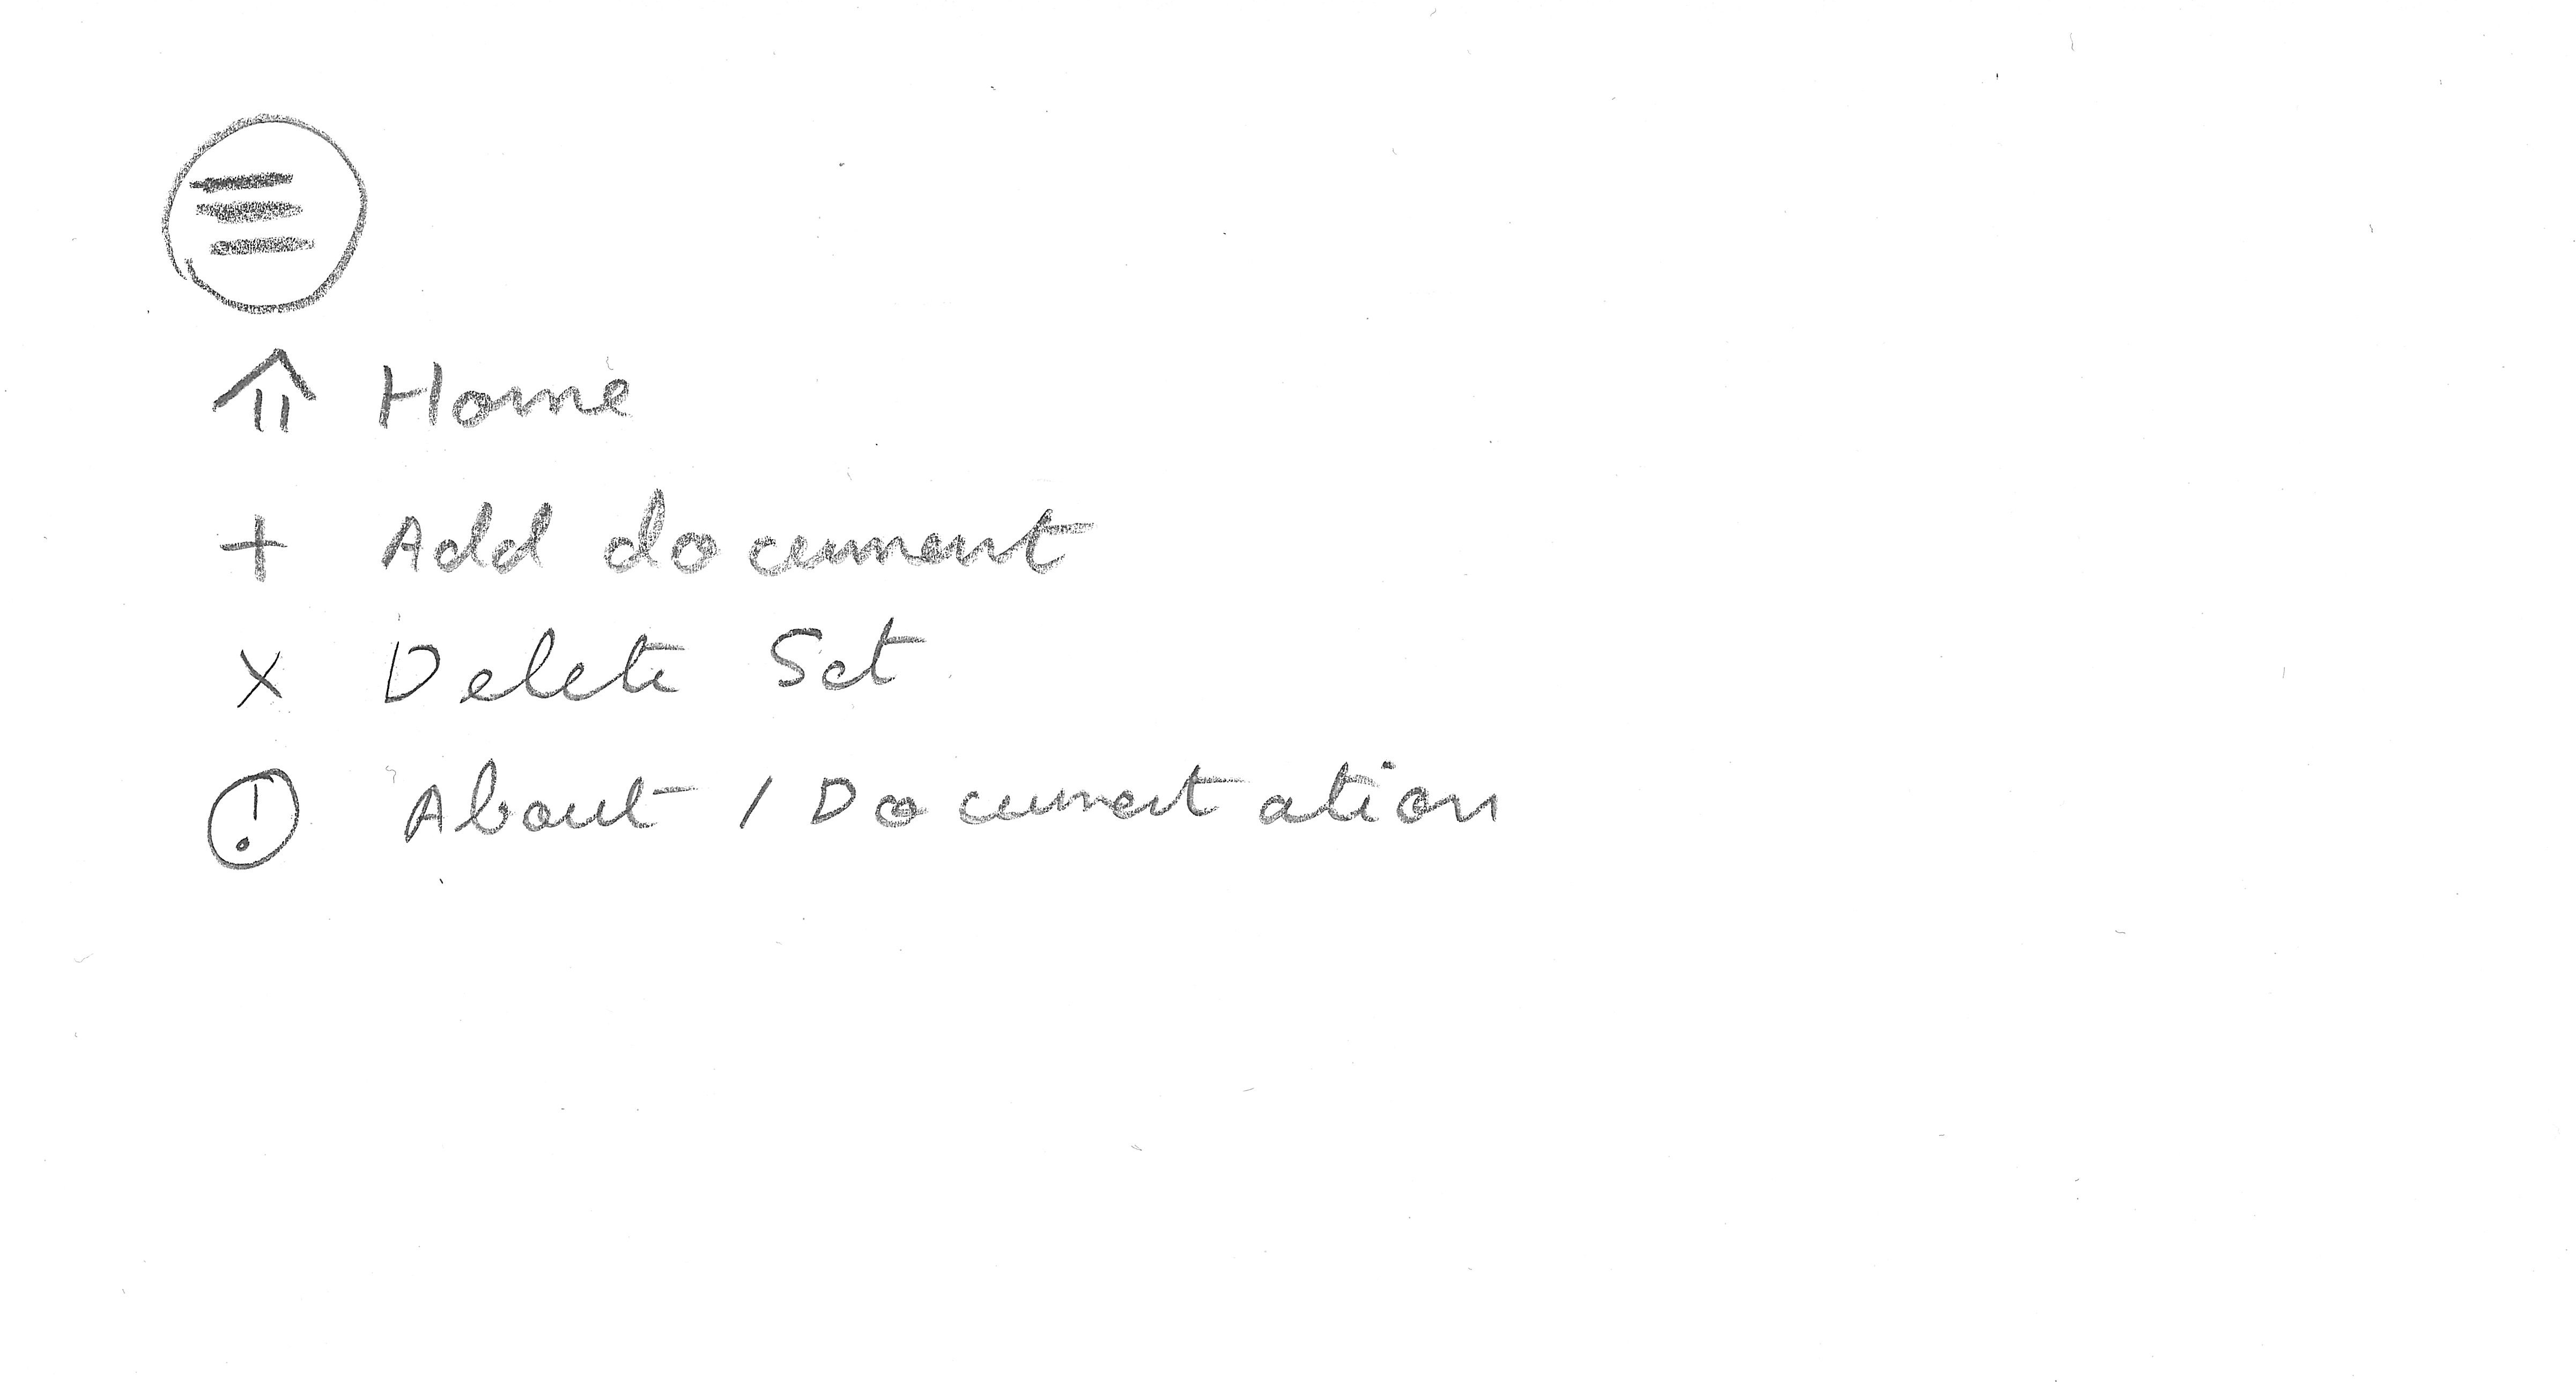
\includegraphics[width=\linewidth]{images/wireframes/set-menu.jpg}
    \end{figure}
    \section{Document View v1}
    \begin{figure}[H]
        \centering
        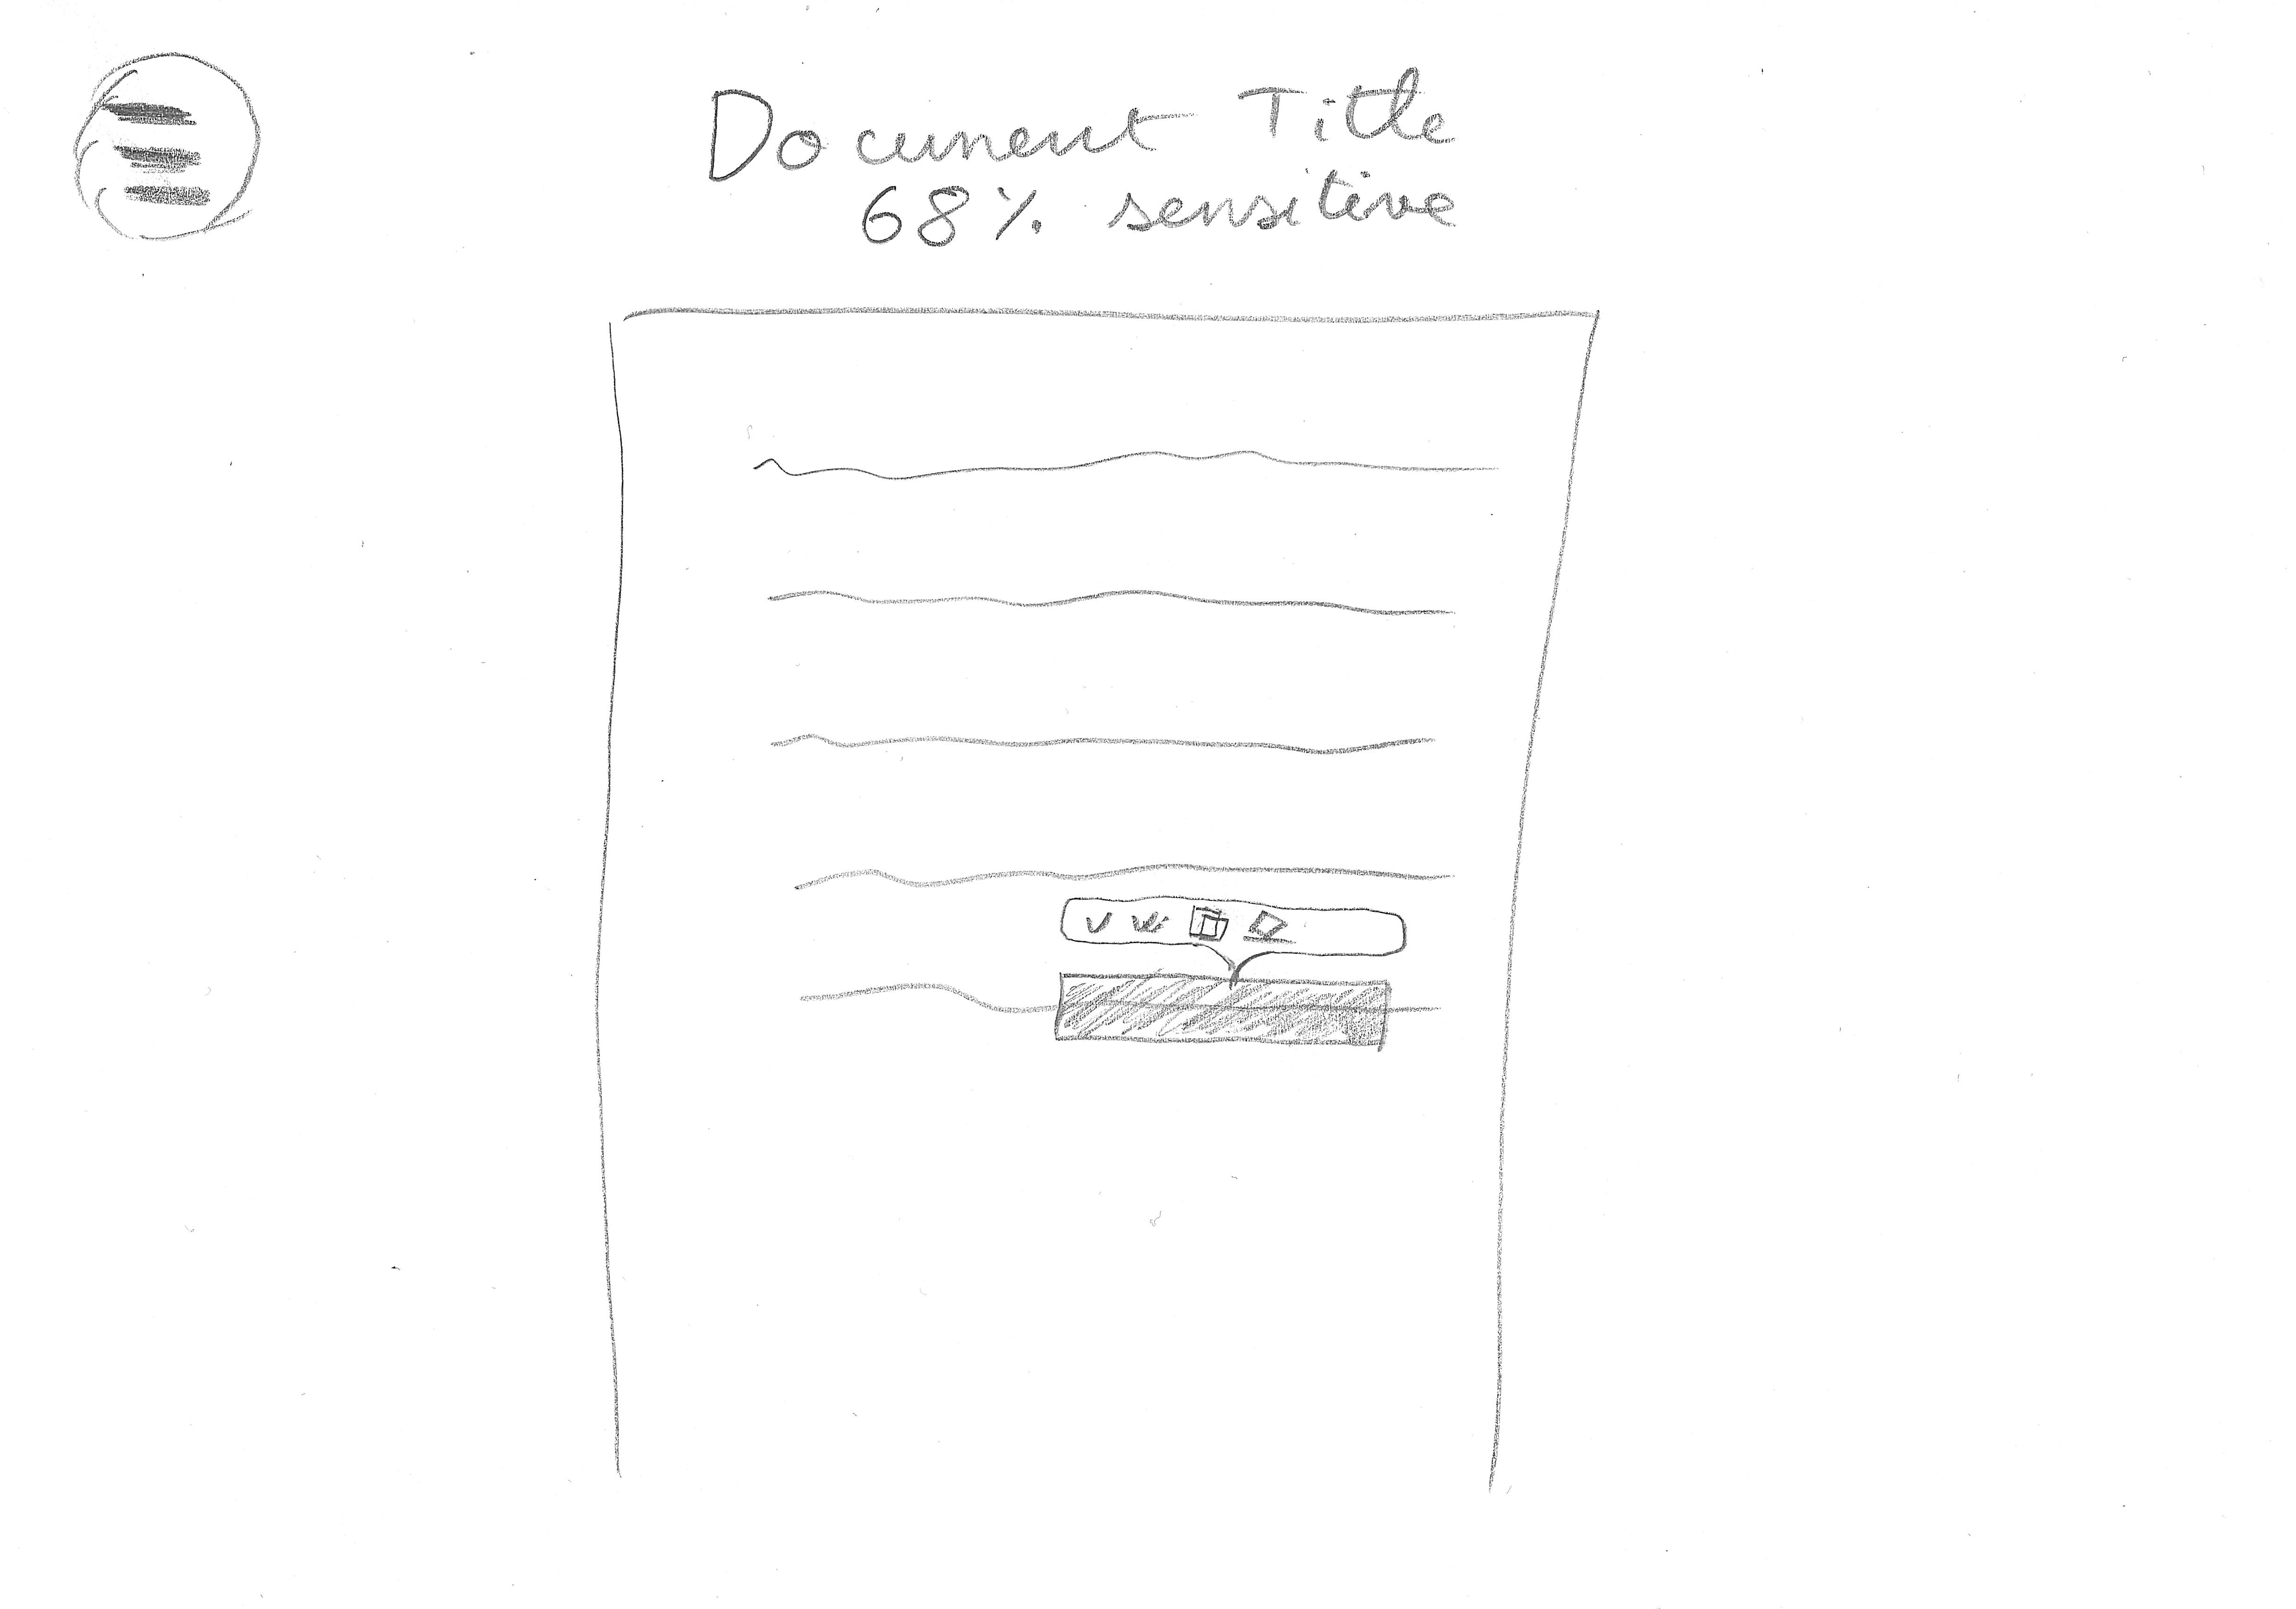
\includegraphics[width=\linewidth]{images/wireframes/page.png}
    \end{figure}
    \section{Document View v2 - opened settings drawer}
    \begin{figure}[H]
        \centering
        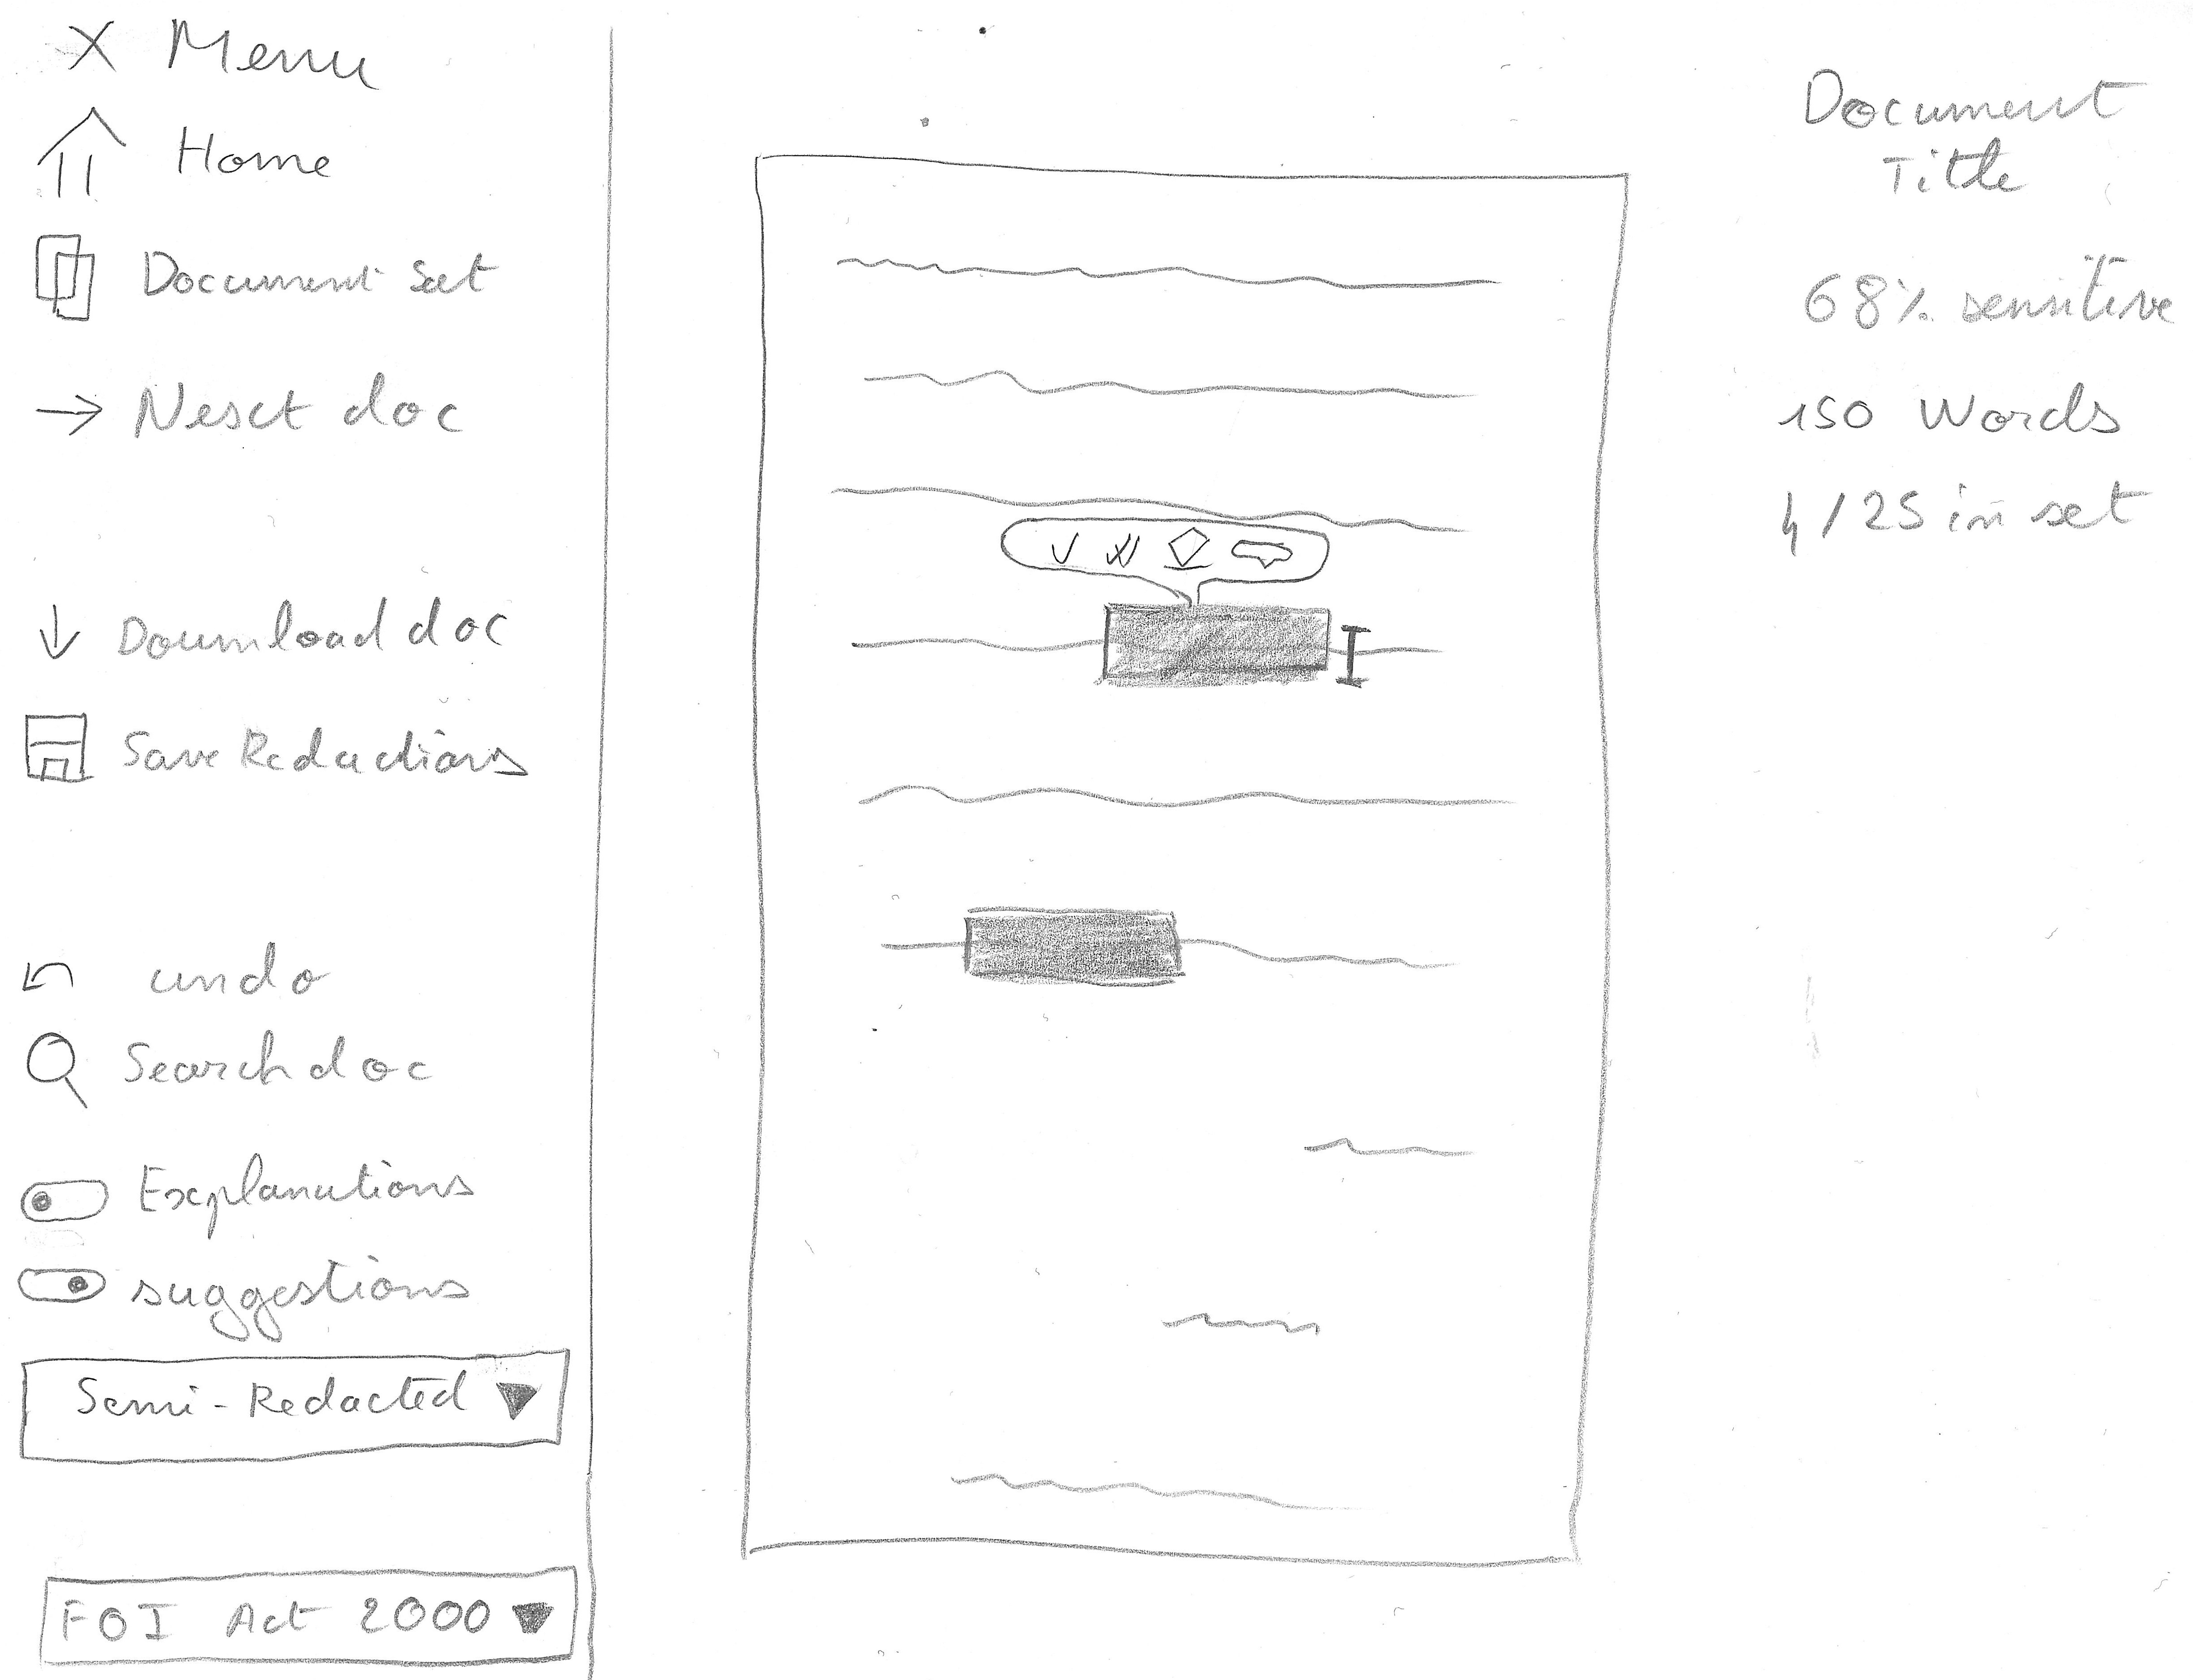
\includegraphics[width=\linewidth]{images/wireframes/doc_view.jpg}
    \end{figure}
    \section{Document View v2 - closed settings drawer}
    \begin{figure}[H]
        \centering
        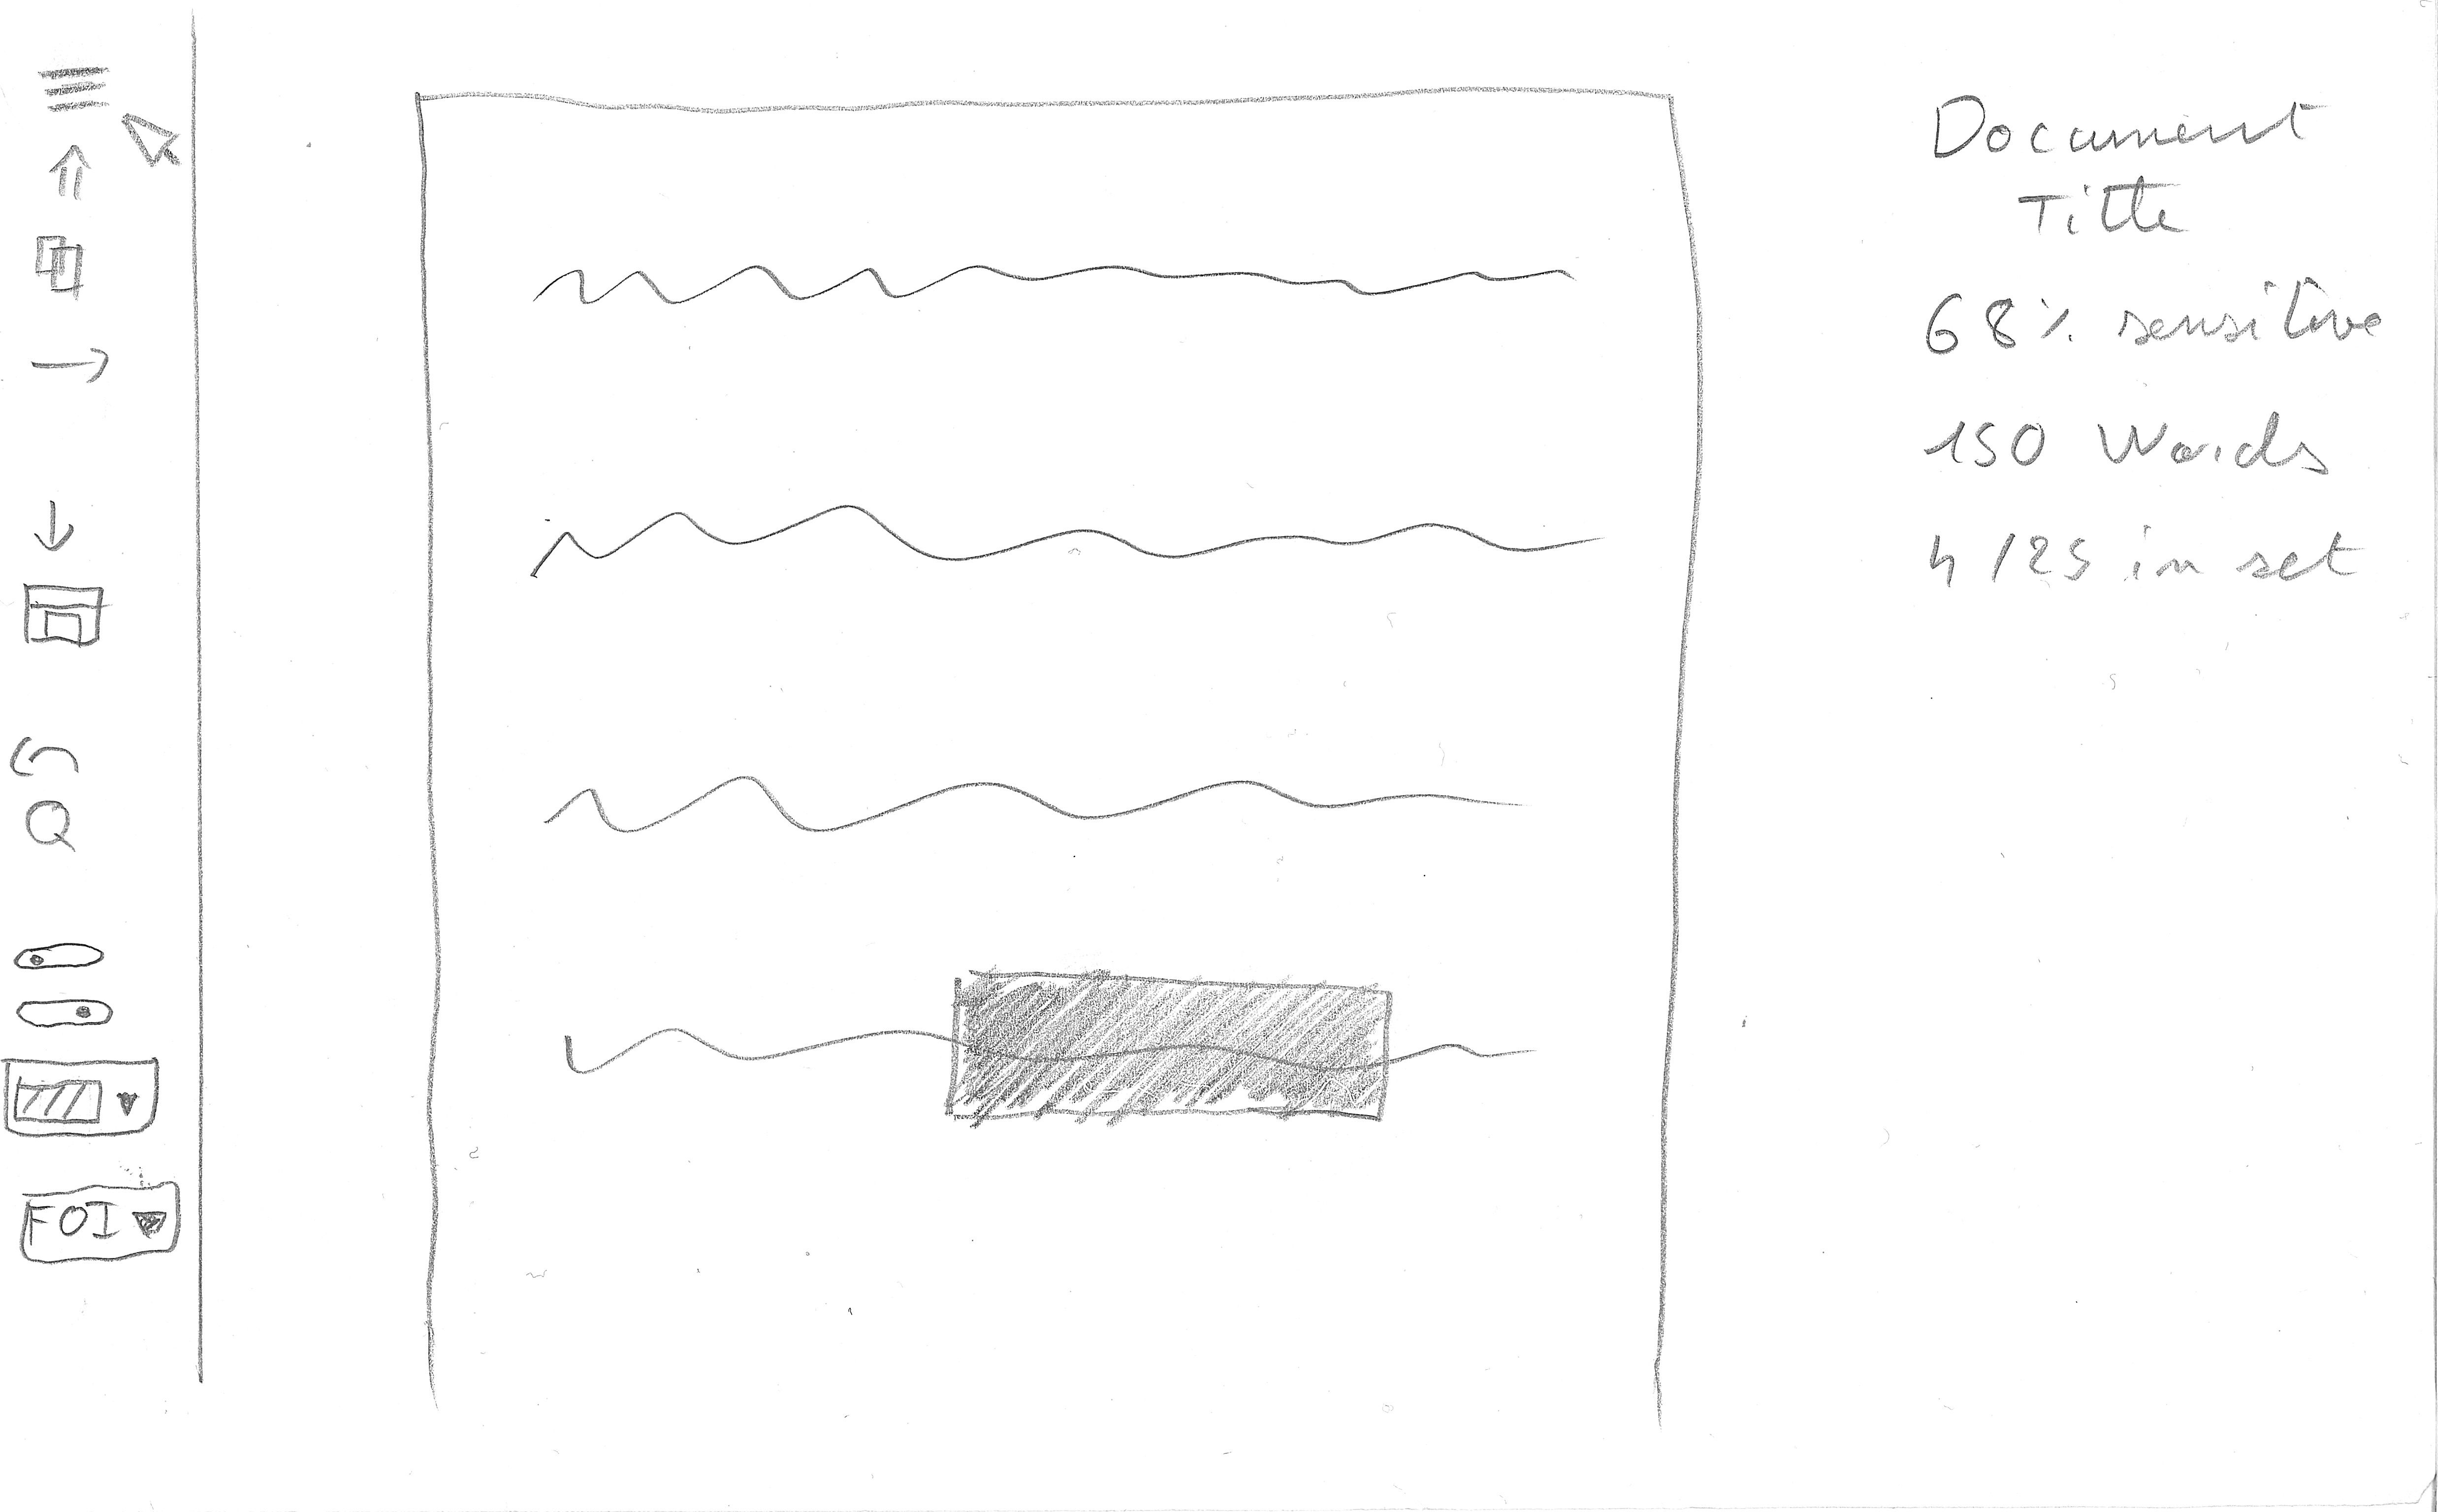
\includegraphics[width=\linewidth]{images/wireframes/doc-view.jpg}
    \end{figure}
    \section{Text Select Tooltip}
    \begin{figure}[H]
        \centering
        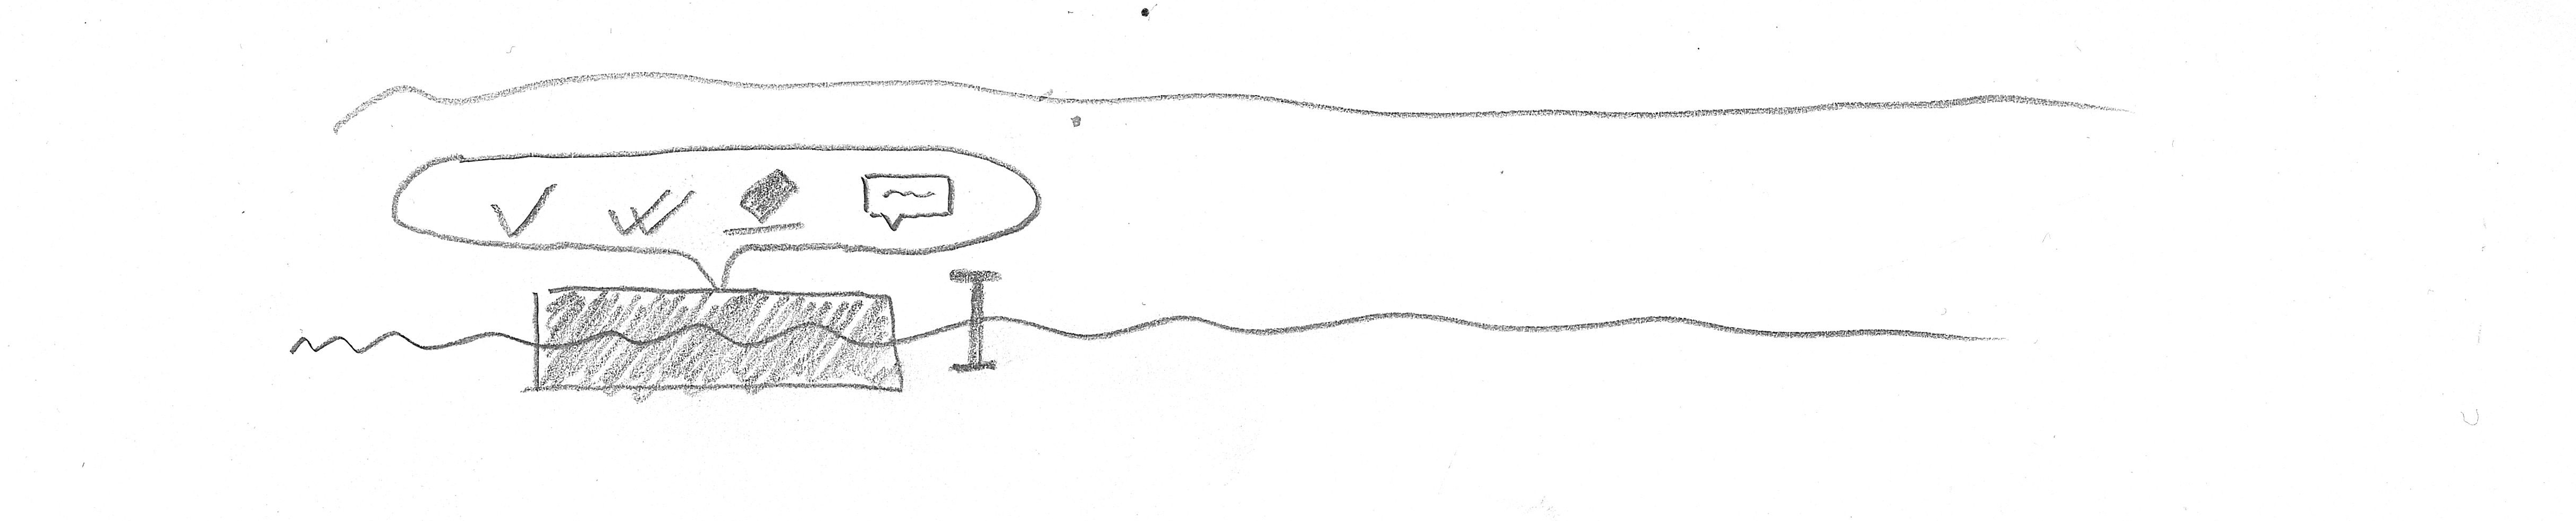
\includegraphics[width=\linewidth]{images/wireframes/tooltip.jpg}
    \end{figure}
    \section{Text Select Tooltip - Opened Comment menu}
    \begin{figure}[H]
        \centering
        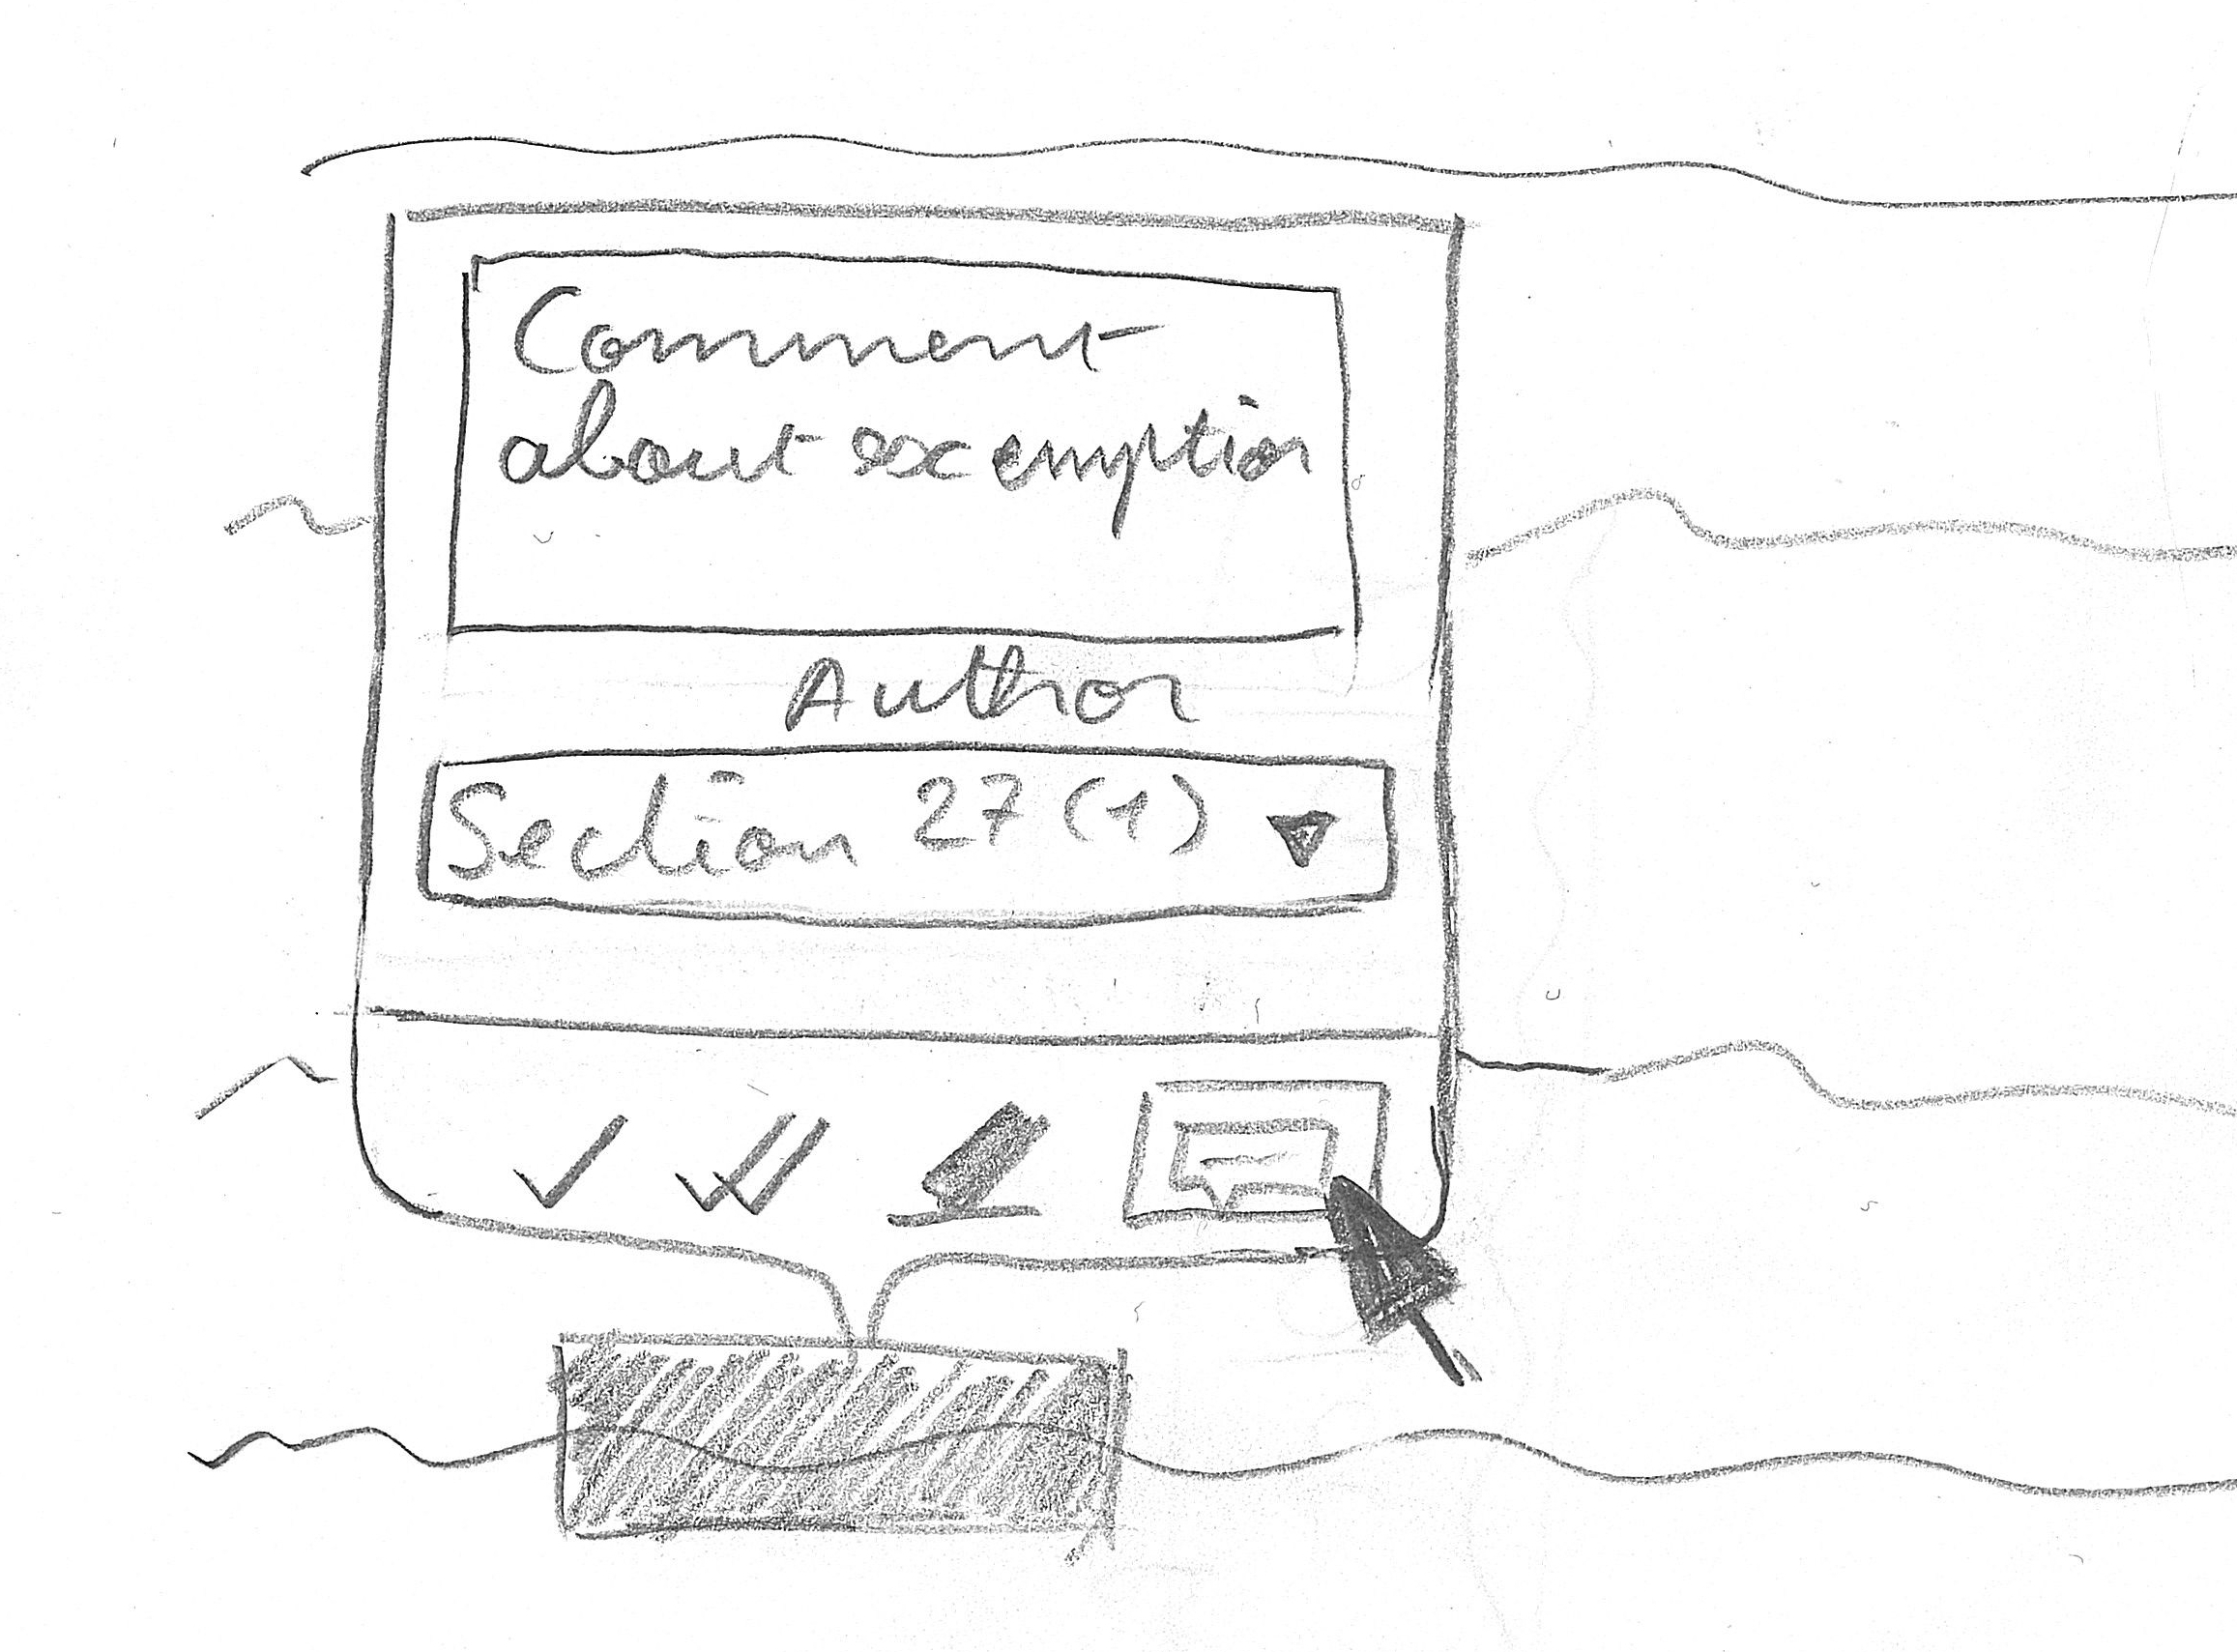
\includegraphics[width=\linewidth]{images/wireframes/tooltip_comment.jpg}
    \end{figure}
    \section{API Documentation}
    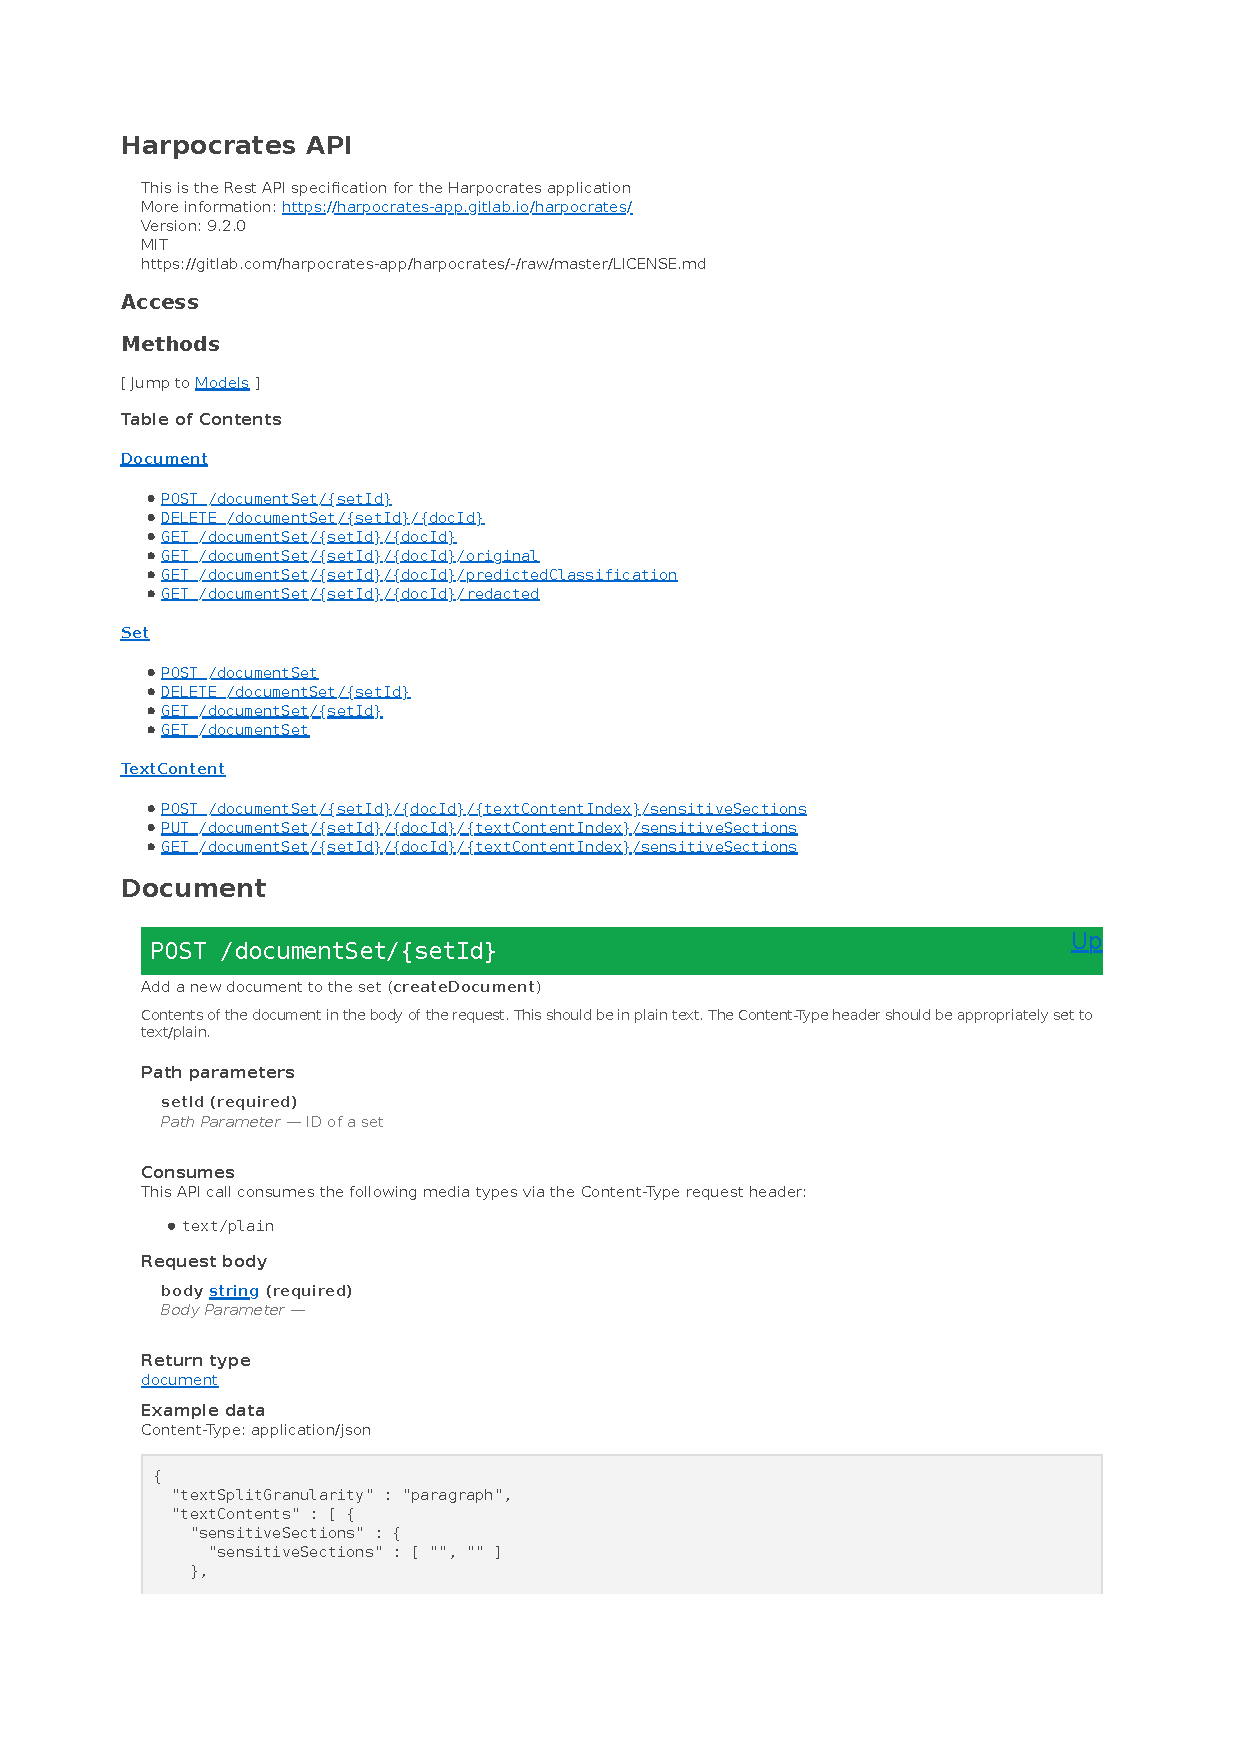
\includepdf[pages={-}]{appendices/api_documentation.pdf}
\end{appendices}
%==================================================================================================================================
%   BIBLIOGRAPHY   


\newpage


\section*{References}

\printbibliography[heading=none]

\vspace*{\fill}
% print license
\doclicenseThis

\end{document}
